\PassOptionsToPackage{unicode=true}{hyperref} % options for packages loaded elsewhere
\PassOptionsToPackage{hyphens}{url}
%
\documentclass[ignorenonframetext,aspectratio=43]{beamer}
\usepackage{pgfpages}
\setbeamertemplate{caption}[numbered]
\setbeamertemplate{caption label separator}{: }
\setbeamercolor{caption name}{fg=normal text.fg}
\beamertemplatenavigationsymbolsempty
% Prevent slide breaks in the middle of a paragraph:
\widowpenalties 1 10000
\raggedbottom
\setbeamertemplate{part page}{
\centering
\begin{beamercolorbox}[sep=16pt,center]{part title}
  \usebeamerfont{part title}\insertpart\par
\end{beamercolorbox}
}
\setbeamertemplate{section page}{
\centering
\begin{beamercolorbox}[sep=12pt,center]{part title}
  \usebeamerfont{section title}\insertsection\par
\end{beamercolorbox}
}
\setbeamertemplate{subsection page}{
\centering
\begin{beamercolorbox}[sep=8pt,center]{part title}
  \usebeamerfont{subsection title}\insertsubsection\par
\end{beamercolorbox}
}
\AtBeginPart{
  \frame{\partpage}
}
\AtBeginSection{
  \ifbibliography
  \else
    \frame{\sectionpage}
  \fi
}
\AtBeginSubsection{
  \frame{\subsectionpage}
}
\usepackage{lmodern}
\usepackage{amssymb,amsmath}
\usepackage{ifxetex,ifluatex}
\usepackage{fixltx2e} % provides \textsubscript
\ifnum 0\ifxetex 1\fi\ifluatex 1\fi=0 % if pdftex
  \usepackage[T1]{fontenc}
  \usepackage[utf8]{inputenc}
  \usepackage{textcomp} % provides euro and other symbols
\else % if luatex or xelatex
  \usepackage{unicode-math}
  \defaultfontfeatures{Ligatures=TeX,Scale=MatchLowercase}
\fi
\usecolortheme{beaver}
% use upquote if available, for straight quotes in verbatim environments
\IfFileExists{upquote.sty}{\usepackage{upquote}}{}
% use microtype if available
\IfFileExists{microtype.sty}{%
\usepackage[]{microtype}
\UseMicrotypeSet[protrusion]{basicmath} % disable protrusion for tt fonts
}{}
\IfFileExists{parskip.sty}{%
\usepackage{parskip}
}{% else
\setlength{\parindent}{0pt}
\setlength{\parskip}{6pt plus 2pt minus 1pt}
}
\usepackage{hyperref}
\hypersetup{
            pdftitle={Missing Data Imputation},
            pdfauthor={Stef van Buuren, University of Utrecht \& TNO},
            pdfborder={0 0 0},
            breaklinks=true}
\urlstyle{same}  % don't use monospace font for urls
\newif\ifbibliography
\usepackage{color}
\usepackage{fancyvrb}
\newcommand{\VerbBar}{|}
\newcommand{\VERB}{\Verb[commandchars=\\\{\}]}
\DefineVerbatimEnvironment{Highlighting}{Verbatim}{commandchars=\\\{\}}
% Add ',fontsize=\small' for more characters per line
\usepackage{framed}
\definecolor{shadecolor}{RGB}{248,248,248}
\newenvironment{Shaded}{\begin{snugshade}}{\end{snugshade}}
\newcommand{\AlertTok}[1]{\textcolor[rgb]{0.94,0.16,0.16}{#1}}
\newcommand{\AnnotationTok}[1]{\textcolor[rgb]{0.56,0.35,0.01}{\textbf{\textit{#1}}}}
\newcommand{\AttributeTok}[1]{\textcolor[rgb]{0.77,0.63,0.00}{#1}}
\newcommand{\BaseNTok}[1]{\textcolor[rgb]{0.00,0.00,0.81}{#1}}
\newcommand{\BuiltInTok}[1]{#1}
\newcommand{\CharTok}[1]{\textcolor[rgb]{0.31,0.60,0.02}{#1}}
\newcommand{\CommentTok}[1]{\textcolor[rgb]{0.56,0.35,0.01}{\textit{#1}}}
\newcommand{\CommentVarTok}[1]{\textcolor[rgb]{0.56,0.35,0.01}{\textbf{\textit{#1}}}}
\newcommand{\ConstantTok}[1]{\textcolor[rgb]{0.00,0.00,0.00}{#1}}
\newcommand{\ControlFlowTok}[1]{\textcolor[rgb]{0.13,0.29,0.53}{\textbf{#1}}}
\newcommand{\DataTypeTok}[1]{\textcolor[rgb]{0.13,0.29,0.53}{#1}}
\newcommand{\DecValTok}[1]{\textcolor[rgb]{0.00,0.00,0.81}{#1}}
\newcommand{\DocumentationTok}[1]{\textcolor[rgb]{0.56,0.35,0.01}{\textbf{\textit{#1}}}}
\newcommand{\ErrorTok}[1]{\textcolor[rgb]{0.64,0.00,0.00}{\textbf{#1}}}
\newcommand{\ExtensionTok}[1]{#1}
\newcommand{\FloatTok}[1]{\textcolor[rgb]{0.00,0.00,0.81}{#1}}
\newcommand{\FunctionTok}[1]{\textcolor[rgb]{0.00,0.00,0.00}{#1}}
\newcommand{\ImportTok}[1]{#1}
\newcommand{\InformationTok}[1]{\textcolor[rgb]{0.56,0.35,0.01}{\textbf{\textit{#1}}}}
\newcommand{\KeywordTok}[1]{\textcolor[rgb]{0.13,0.29,0.53}{\textbf{#1}}}
\newcommand{\NormalTok}[1]{#1}
\newcommand{\OperatorTok}[1]{\textcolor[rgb]{0.81,0.36,0.00}{\textbf{#1}}}
\newcommand{\OtherTok}[1]{\textcolor[rgb]{0.56,0.35,0.01}{#1}}
\newcommand{\PreprocessorTok}[1]{\textcolor[rgb]{0.56,0.35,0.01}{\textit{#1}}}
\newcommand{\RegionMarkerTok}[1]{#1}
\newcommand{\SpecialCharTok}[1]{\textcolor[rgb]{0.00,0.00,0.00}{#1}}
\newcommand{\SpecialStringTok}[1]{\textcolor[rgb]{0.31,0.60,0.02}{#1}}
\newcommand{\StringTok}[1]{\textcolor[rgb]{0.31,0.60,0.02}{#1}}
\newcommand{\VariableTok}[1]{\textcolor[rgb]{0.00,0.00,0.00}{#1}}
\newcommand{\VerbatimStringTok}[1]{\textcolor[rgb]{0.31,0.60,0.02}{#1}}
\newcommand{\WarningTok}[1]{\textcolor[rgb]{0.56,0.35,0.01}{\textbf{\textit{#1}}}}
\usepackage{longtable,booktabs}
\usepackage{caption}
% These lines are needed to make table captions work with longtable:
\makeatletter
\def\fnum@table{\tablename~\thetable}
\makeatother
\usepackage{graphicx,grffile}
\makeatletter
\def\maxwidth{\ifdim\Gin@nat@width>\linewidth\linewidth\else\Gin@nat@width\fi}
\def\maxheight{\ifdim\Gin@nat@height>\textheight\textheight\else\Gin@nat@height\fi}
\makeatother
% Scale images if necessary, so that they will not overflow the page
% margins by default, and it is still possible to overwrite the defaults
% using explicit options in \includegraphics[width, height, ...]{}
\setkeys{Gin}{width=\maxwidth,height=\maxheight,keepaspectratio}
\setlength{\emergencystretch}{3em}  % prevent overfull lines
\providecommand{\tightlist}{%
  \setlength{\itemsep}{0pt}\setlength{\parskip}{0pt}}
\setcounter{secnumdepth}{0}

% set default figure placement to htbp
\makeatletter
\def\fps@figure{htbp}
\makeatother


\title{Missing Data Imputation}
\providecommand{\subtitle}[1]{}
\subtitle{Applying multiple imputation to survey data harmonized ex-post}
\author{Stef van Buuren, University of Utrecht \& TNO}
\date{December 19, 2019; Building Multi-Source Databases for Comparative
Analyses}

\begin{document}
\frame{\titlepage}

\begin{frame}
\tableofcontents[hideallsubsections]
\end{frame}
\begin{frame}{Two problems in combining datasets}
\protect\hypertarget{two-problems-in-combining-datasets}{}

\begin{enumerate}
\tightlist
\item
  Different number of categories
\item
  Uncollected variables
\end{enumerate}

\end{frame}

\begin{frame}{1. Different number of categories}
\protect\hypertarget{different-number-of-categories}{}

\end{frame}

\begin{frame}{Trust in government}
\protect\hypertarget{trust-in-government}{}

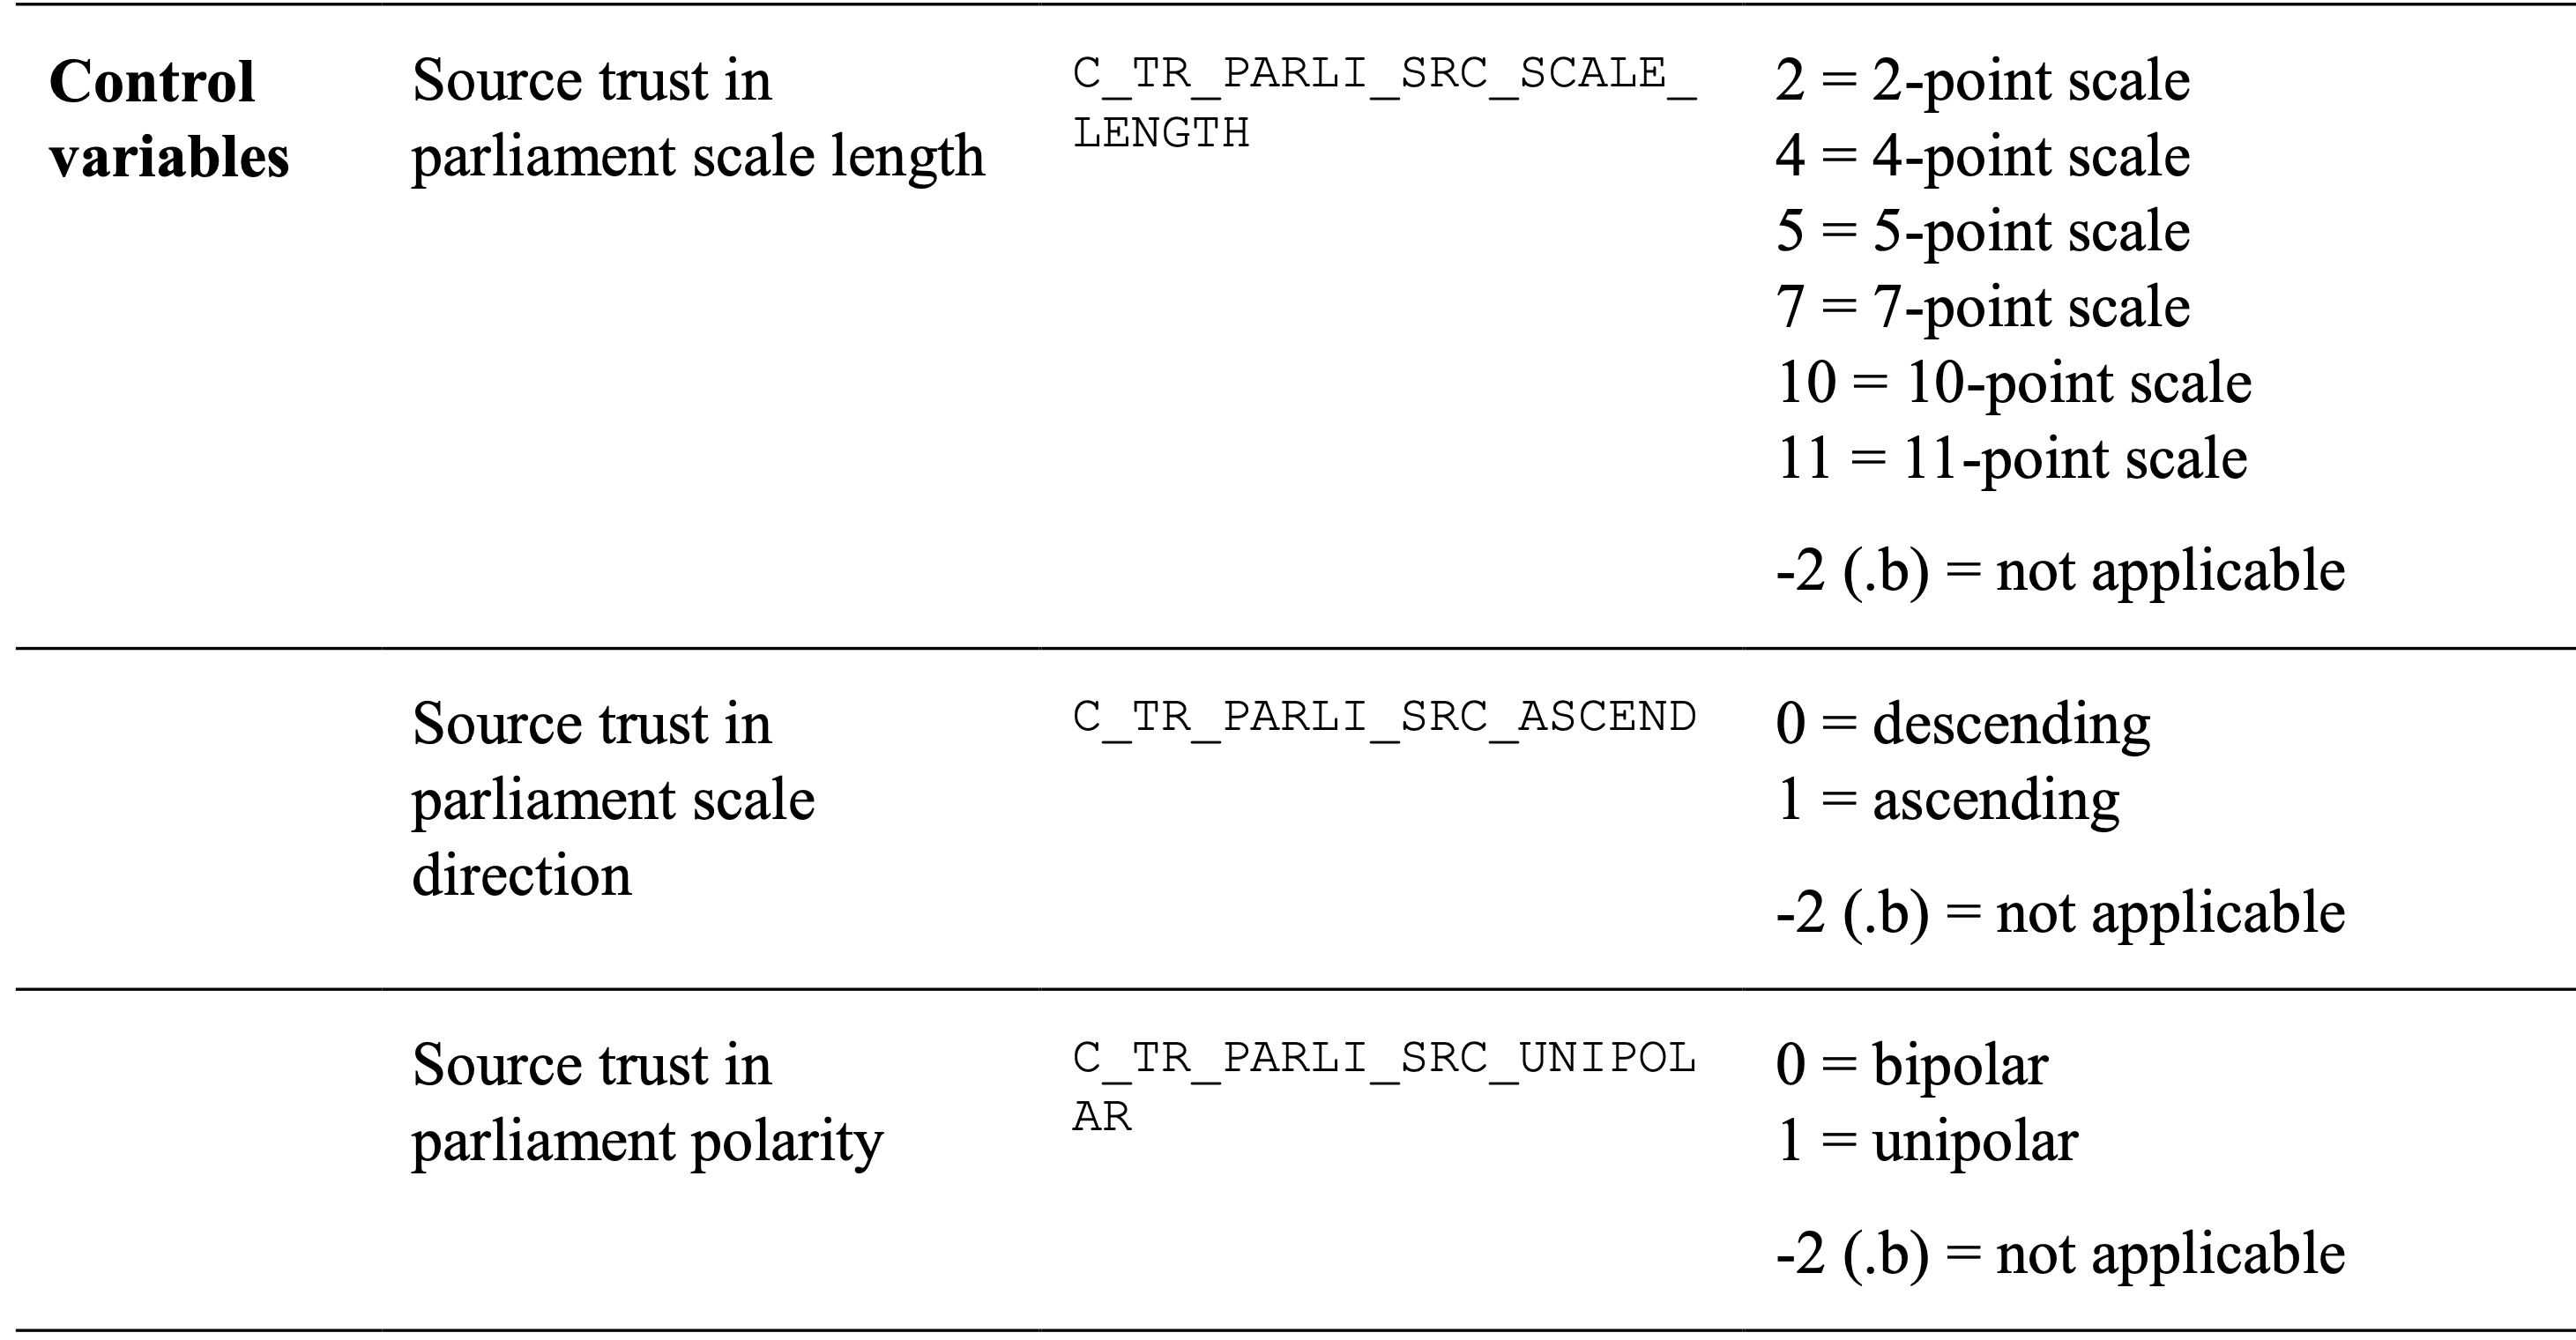
\includegraphics{figures/controlvars.png}

\end{frame}

\begin{frame}{Method 1: Stretch to finer scale}
\protect\hypertarget{method-1-stretch-to-finer-scale}{}

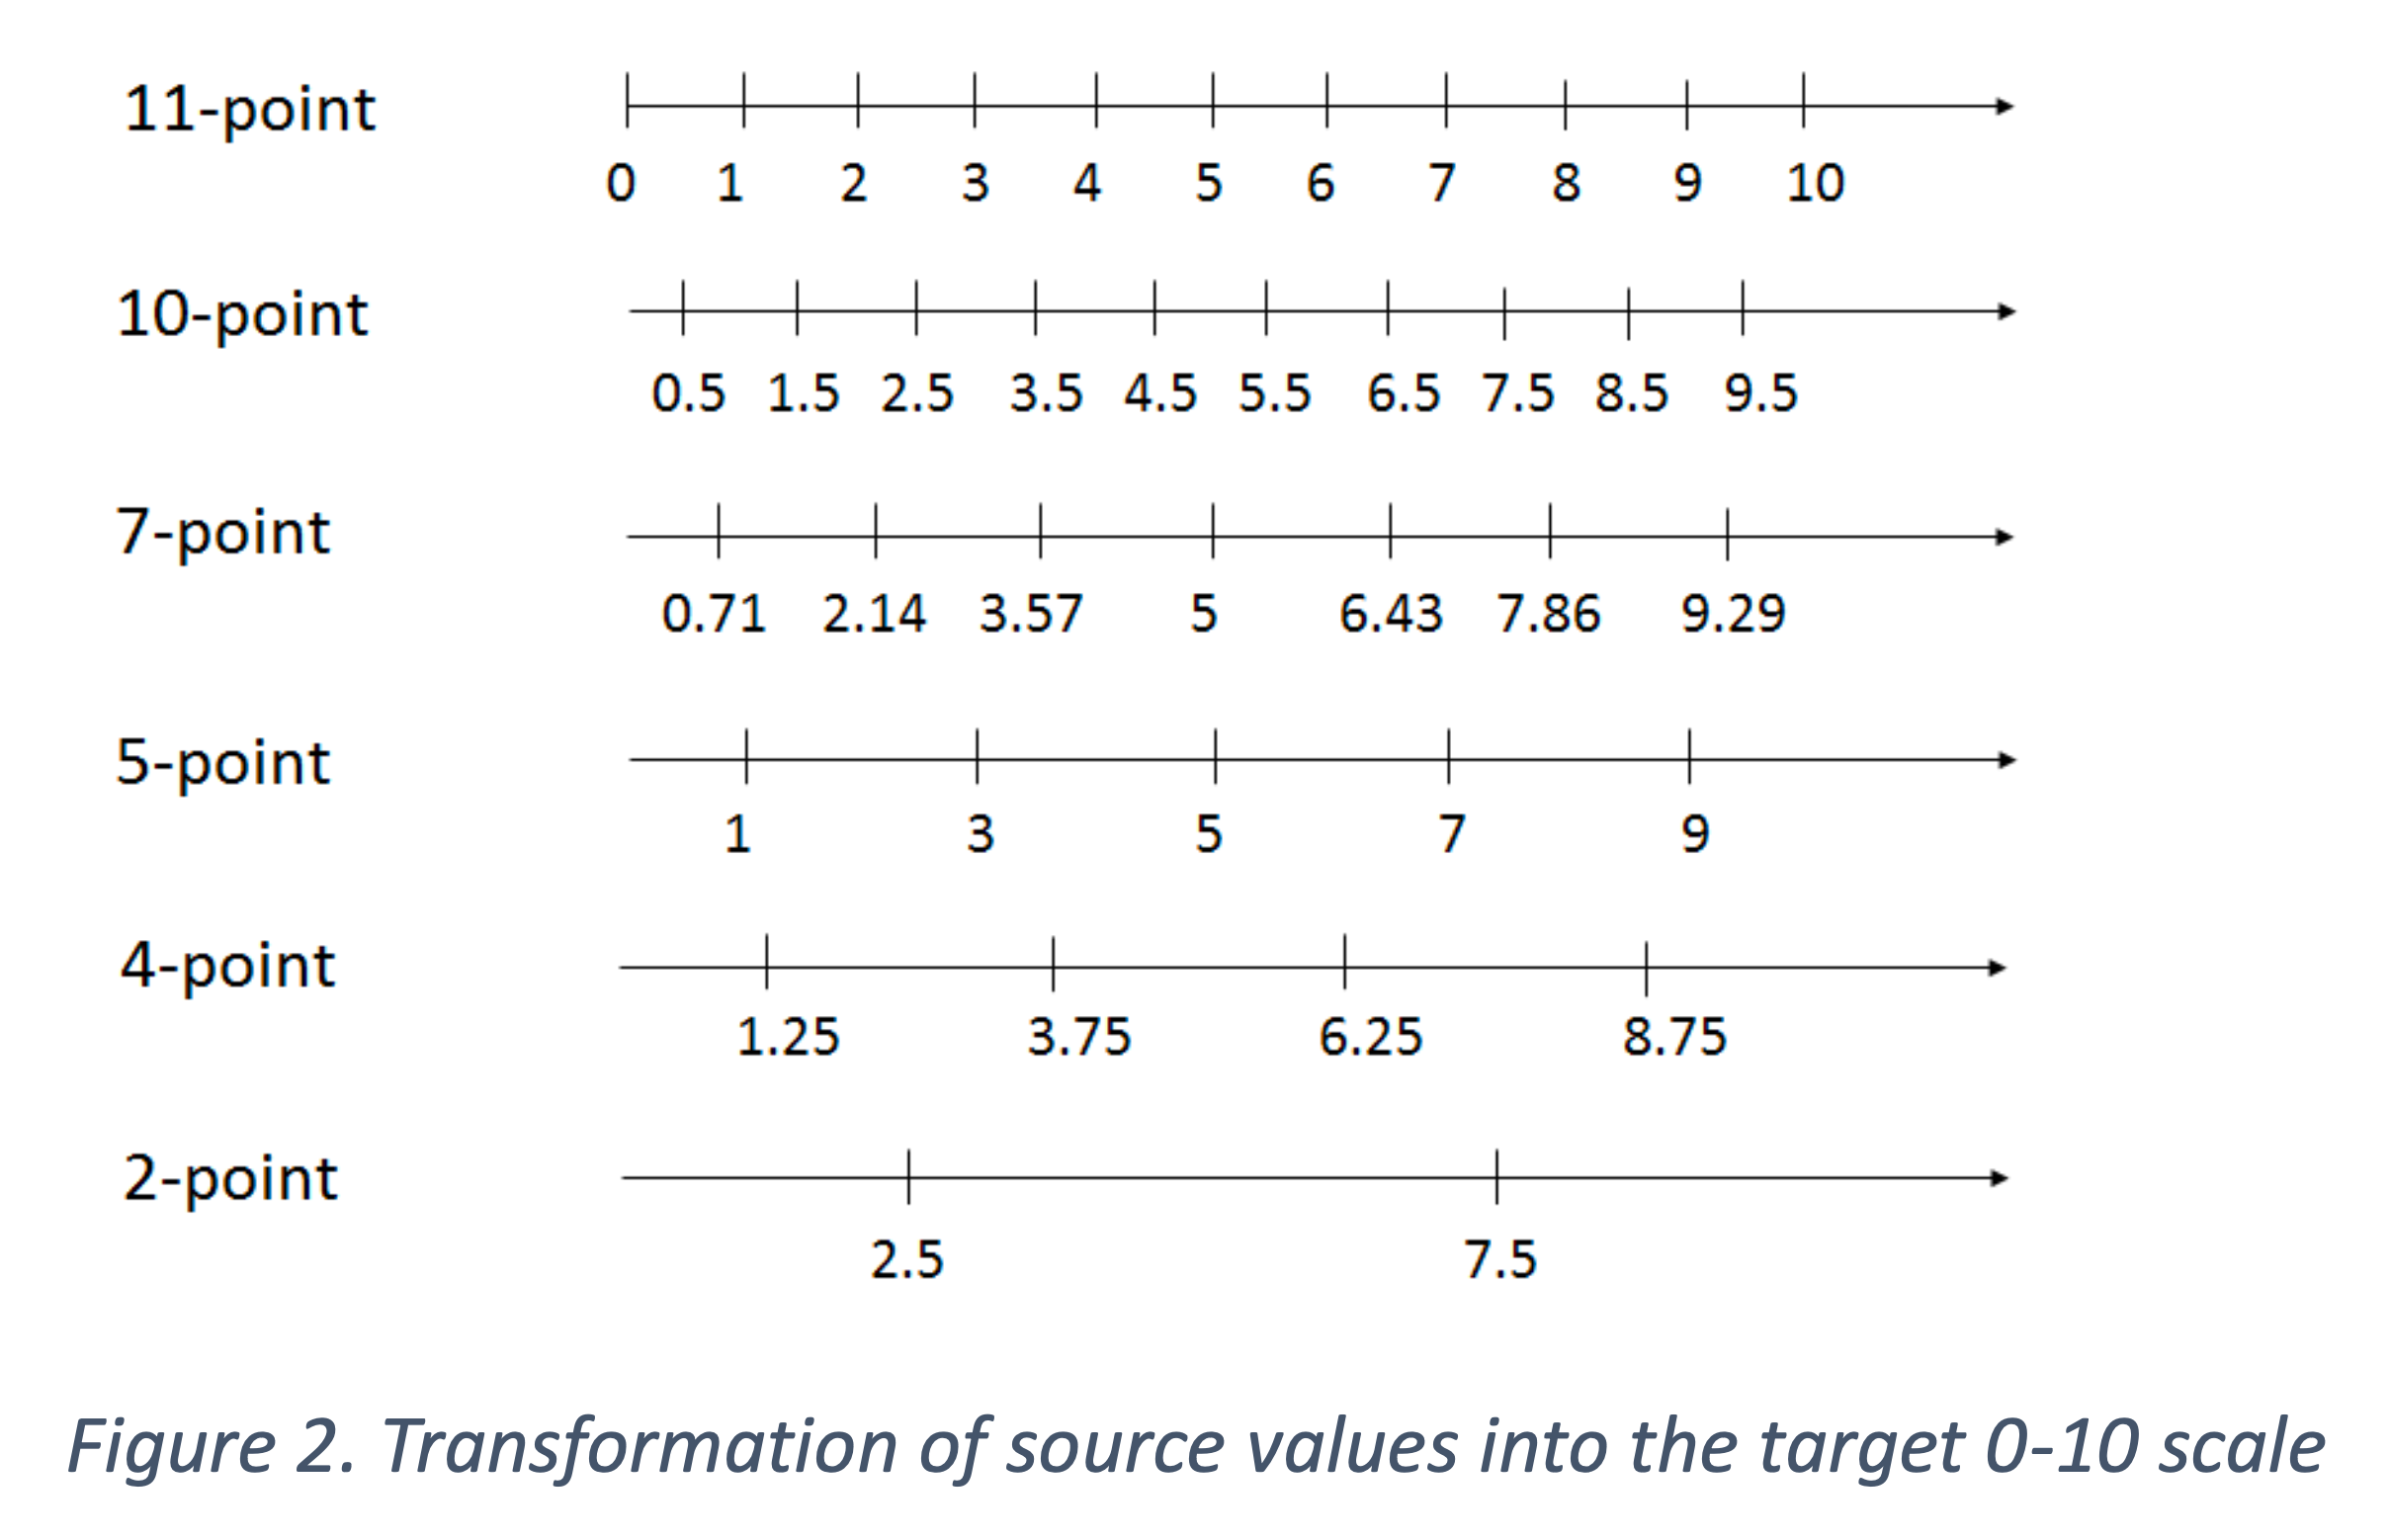
\includegraphics{figures/figure2.png}

\end{frame}

\begin{frame}{Method 2: Align ranges}
\protect\hypertarget{method-2-align-ranges}{}

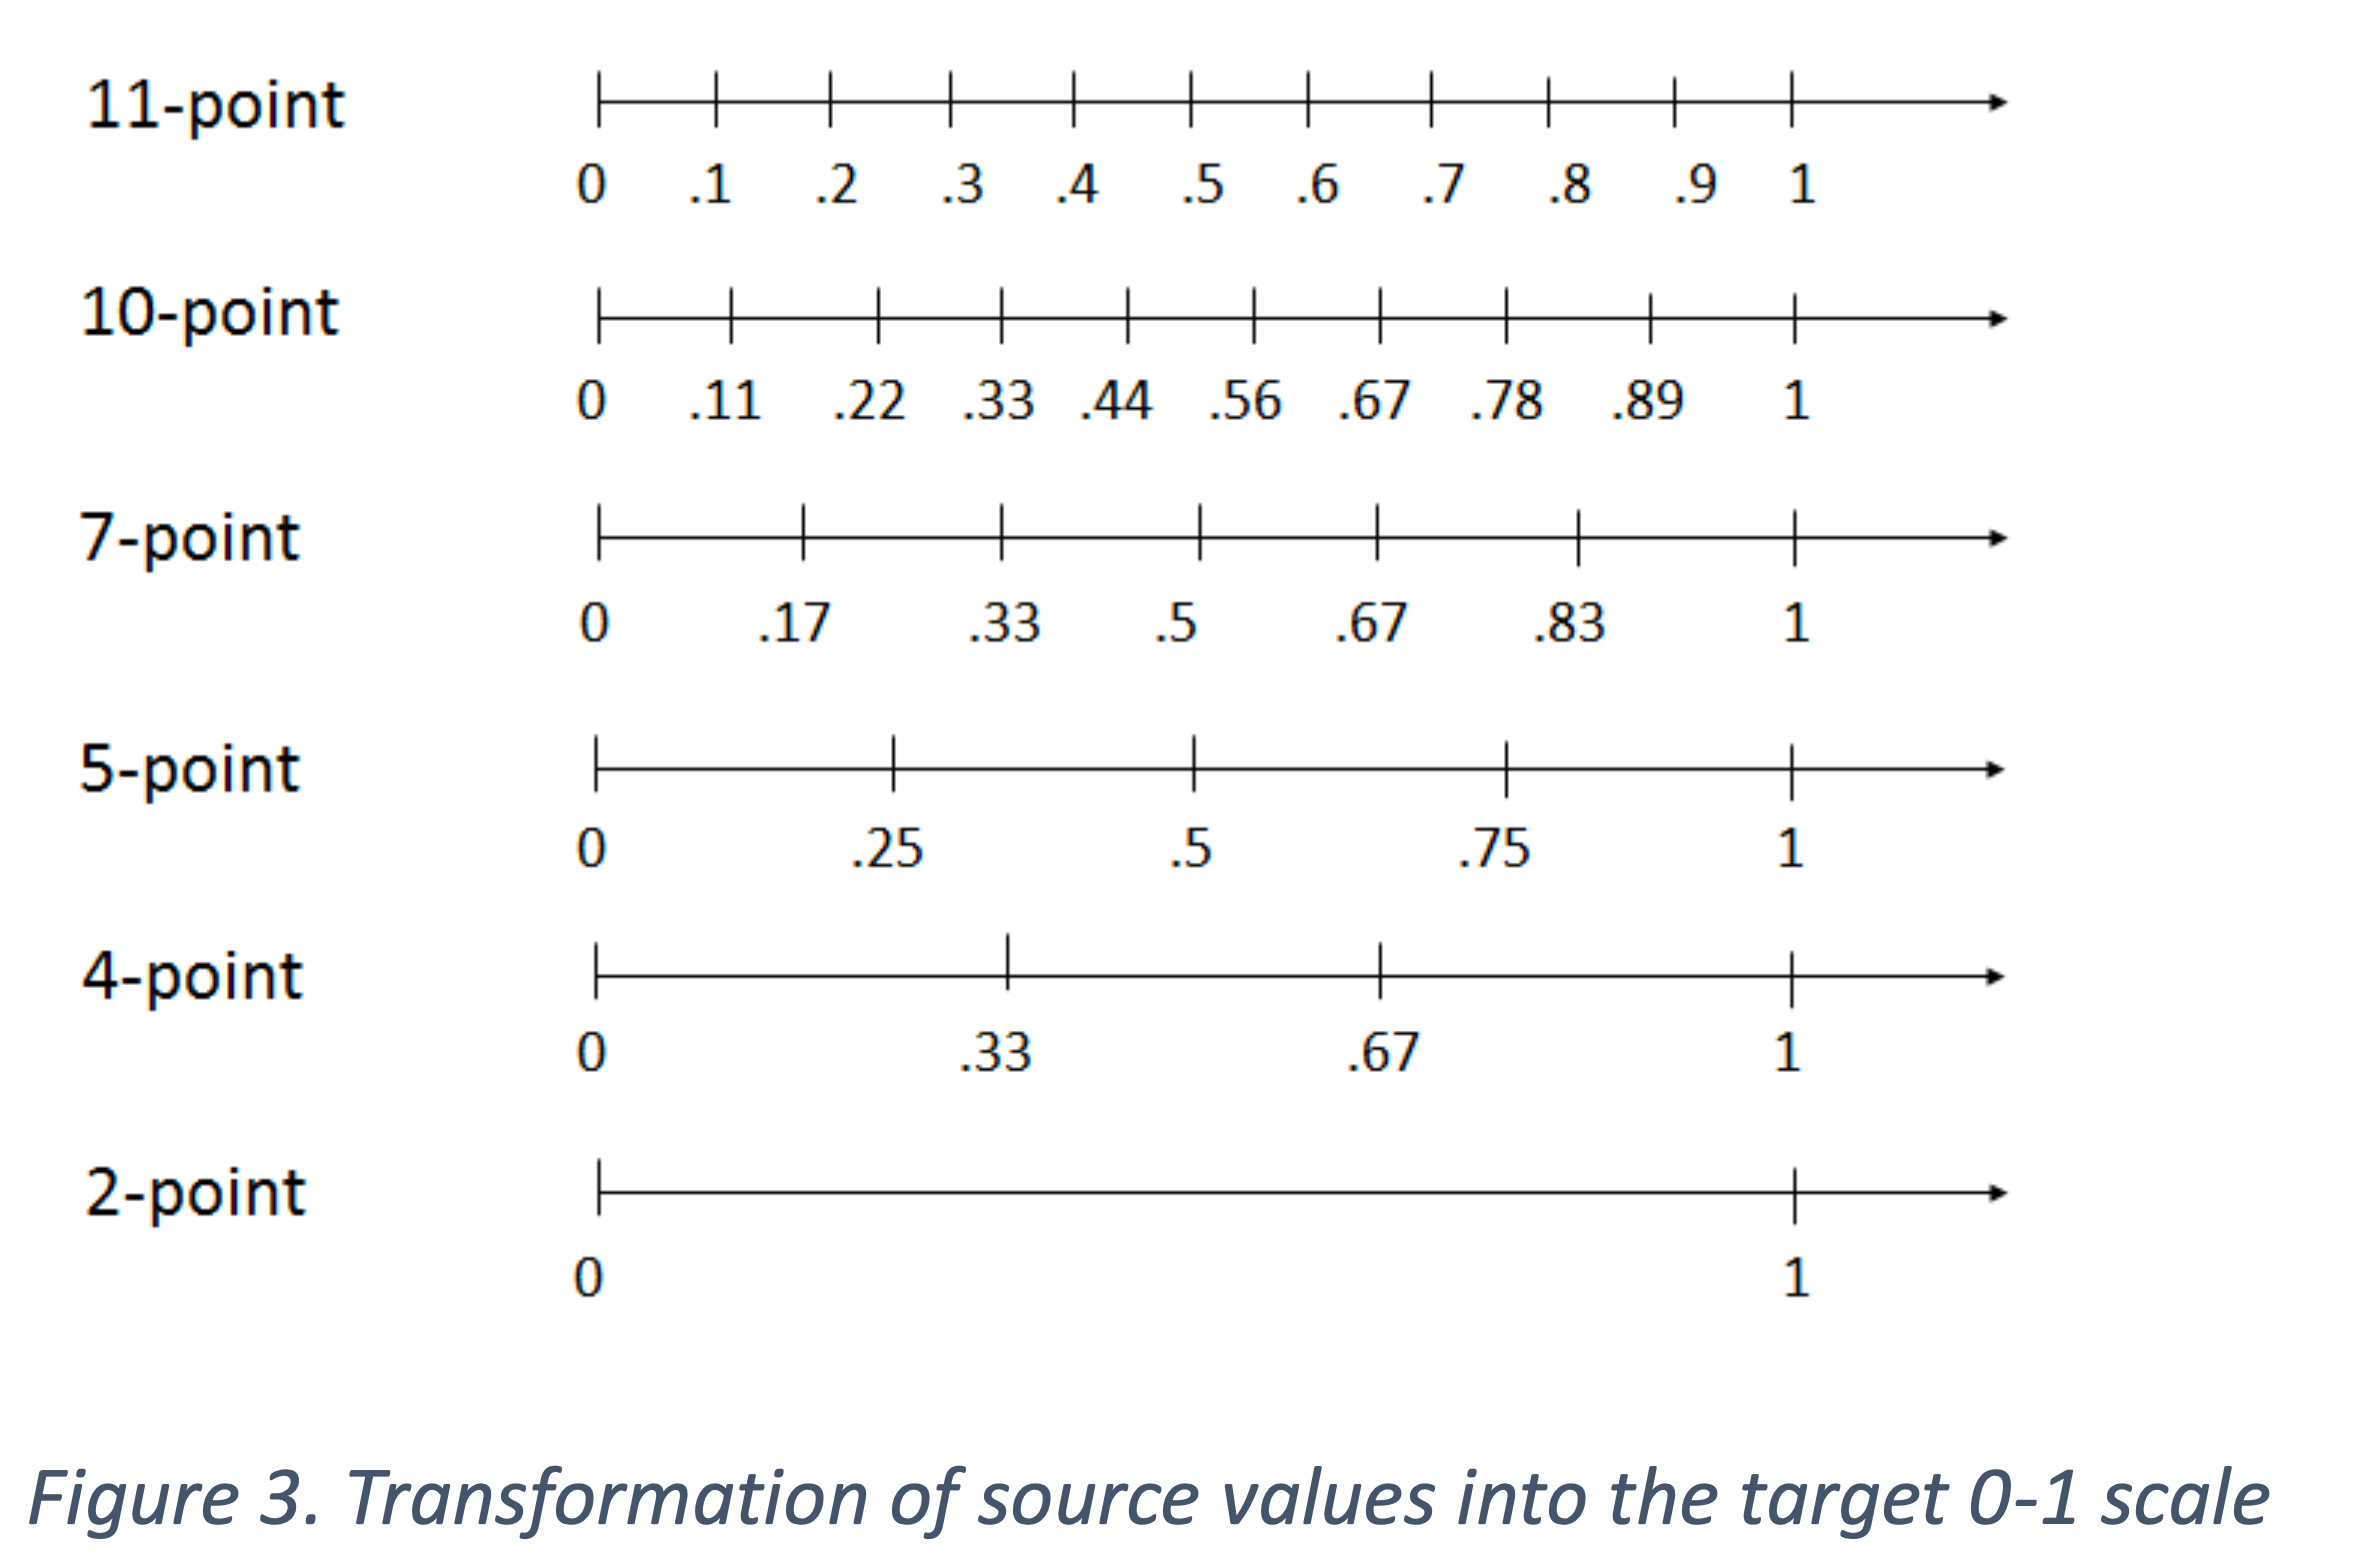
\includegraphics{figures/figure3.png}

\end{frame}

\begin{frame}{Method 3: Cohortwise transform to uniform}
\protect\hypertarget{method-3-cohortwise-transform-to-uniform}{}

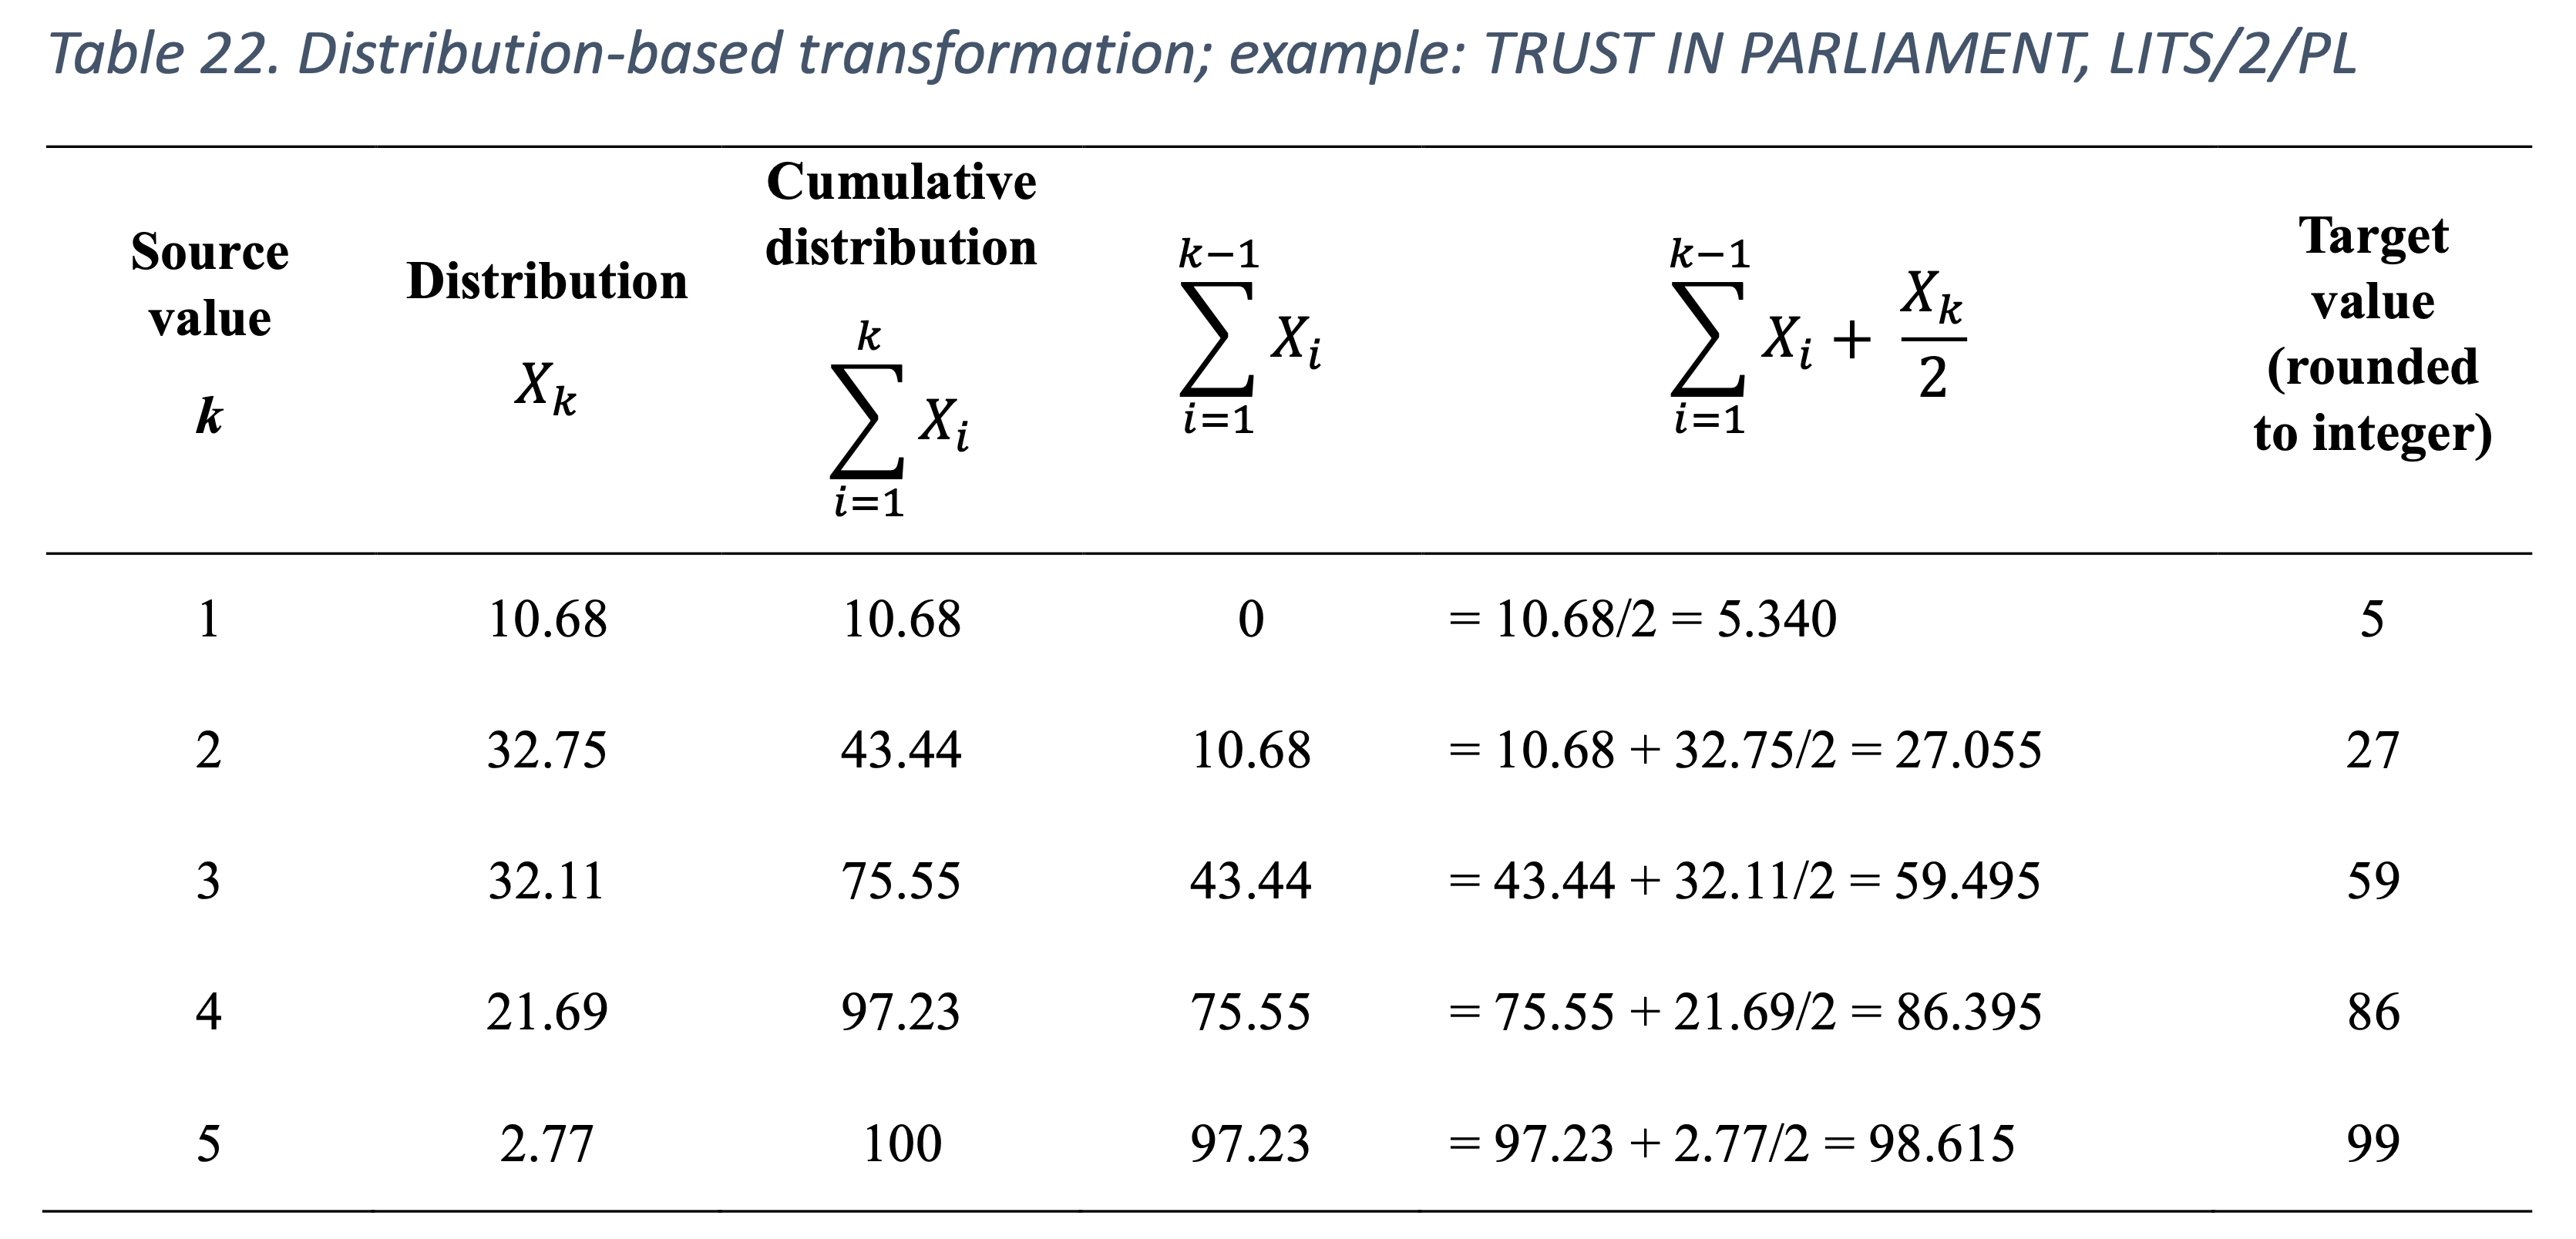
\includegraphics{figures/figure22.png}

\end{frame}

\begin{frame}{1 vs 2}
\protect\hypertarget{vs-2}{}

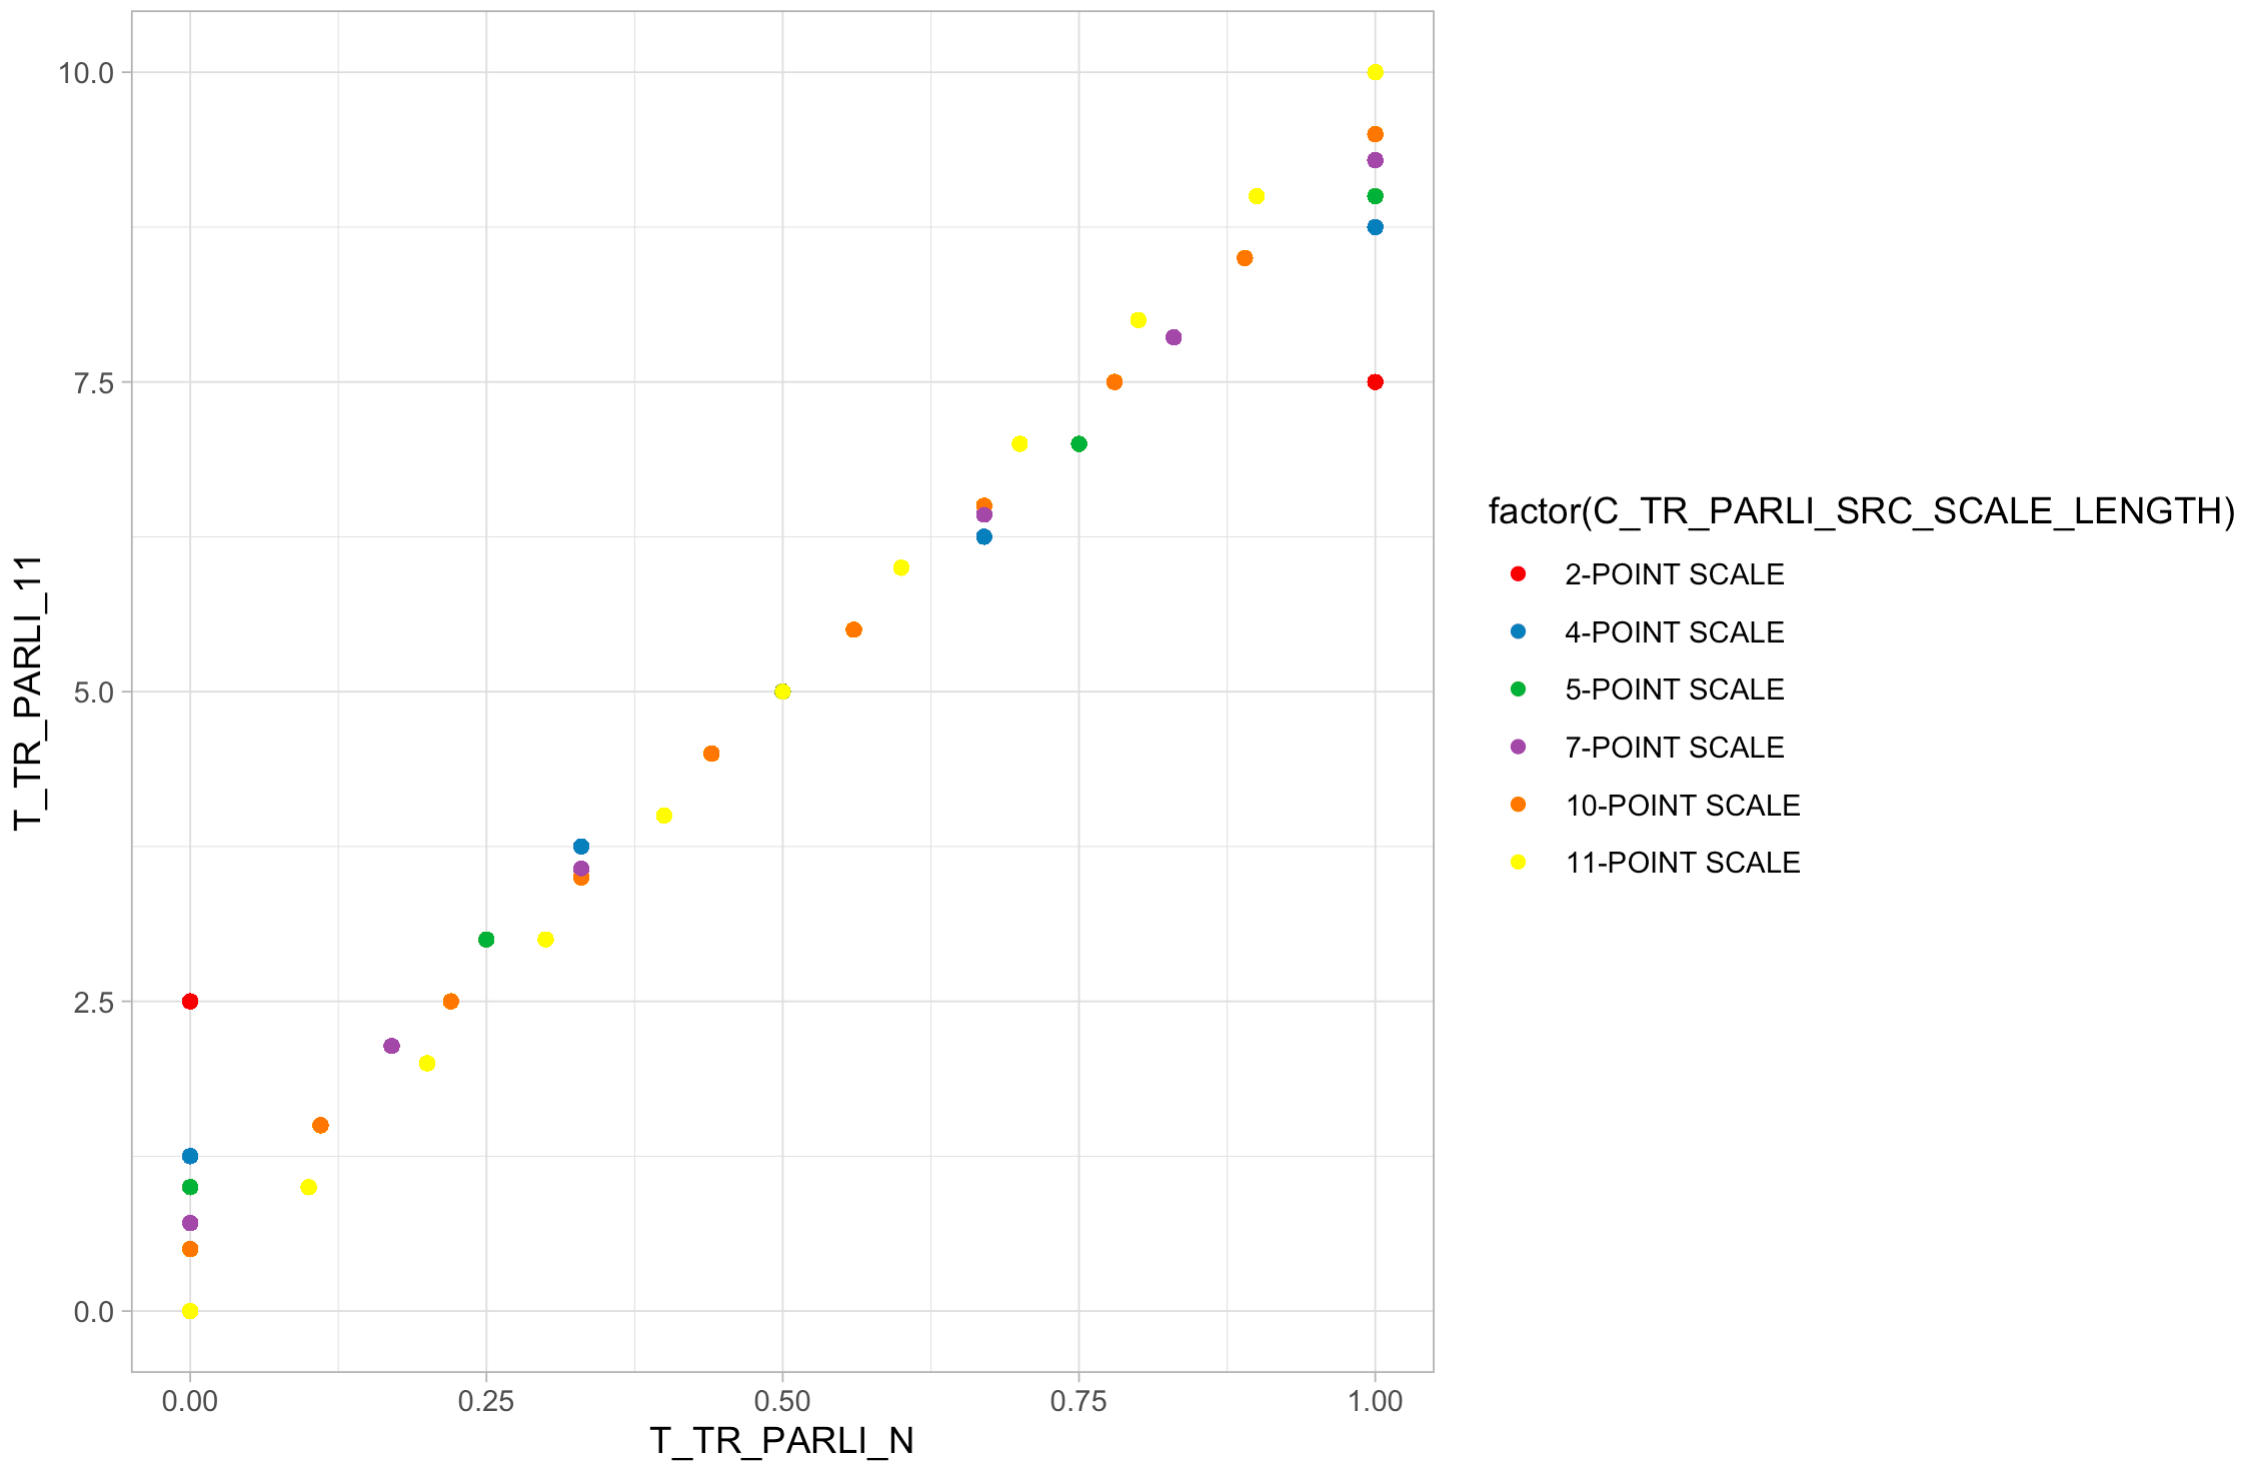
\includegraphics{figures/scatter1.png}

\end{frame}

\begin{frame}{1 vs 3}
\protect\hypertarget{vs-3}{}

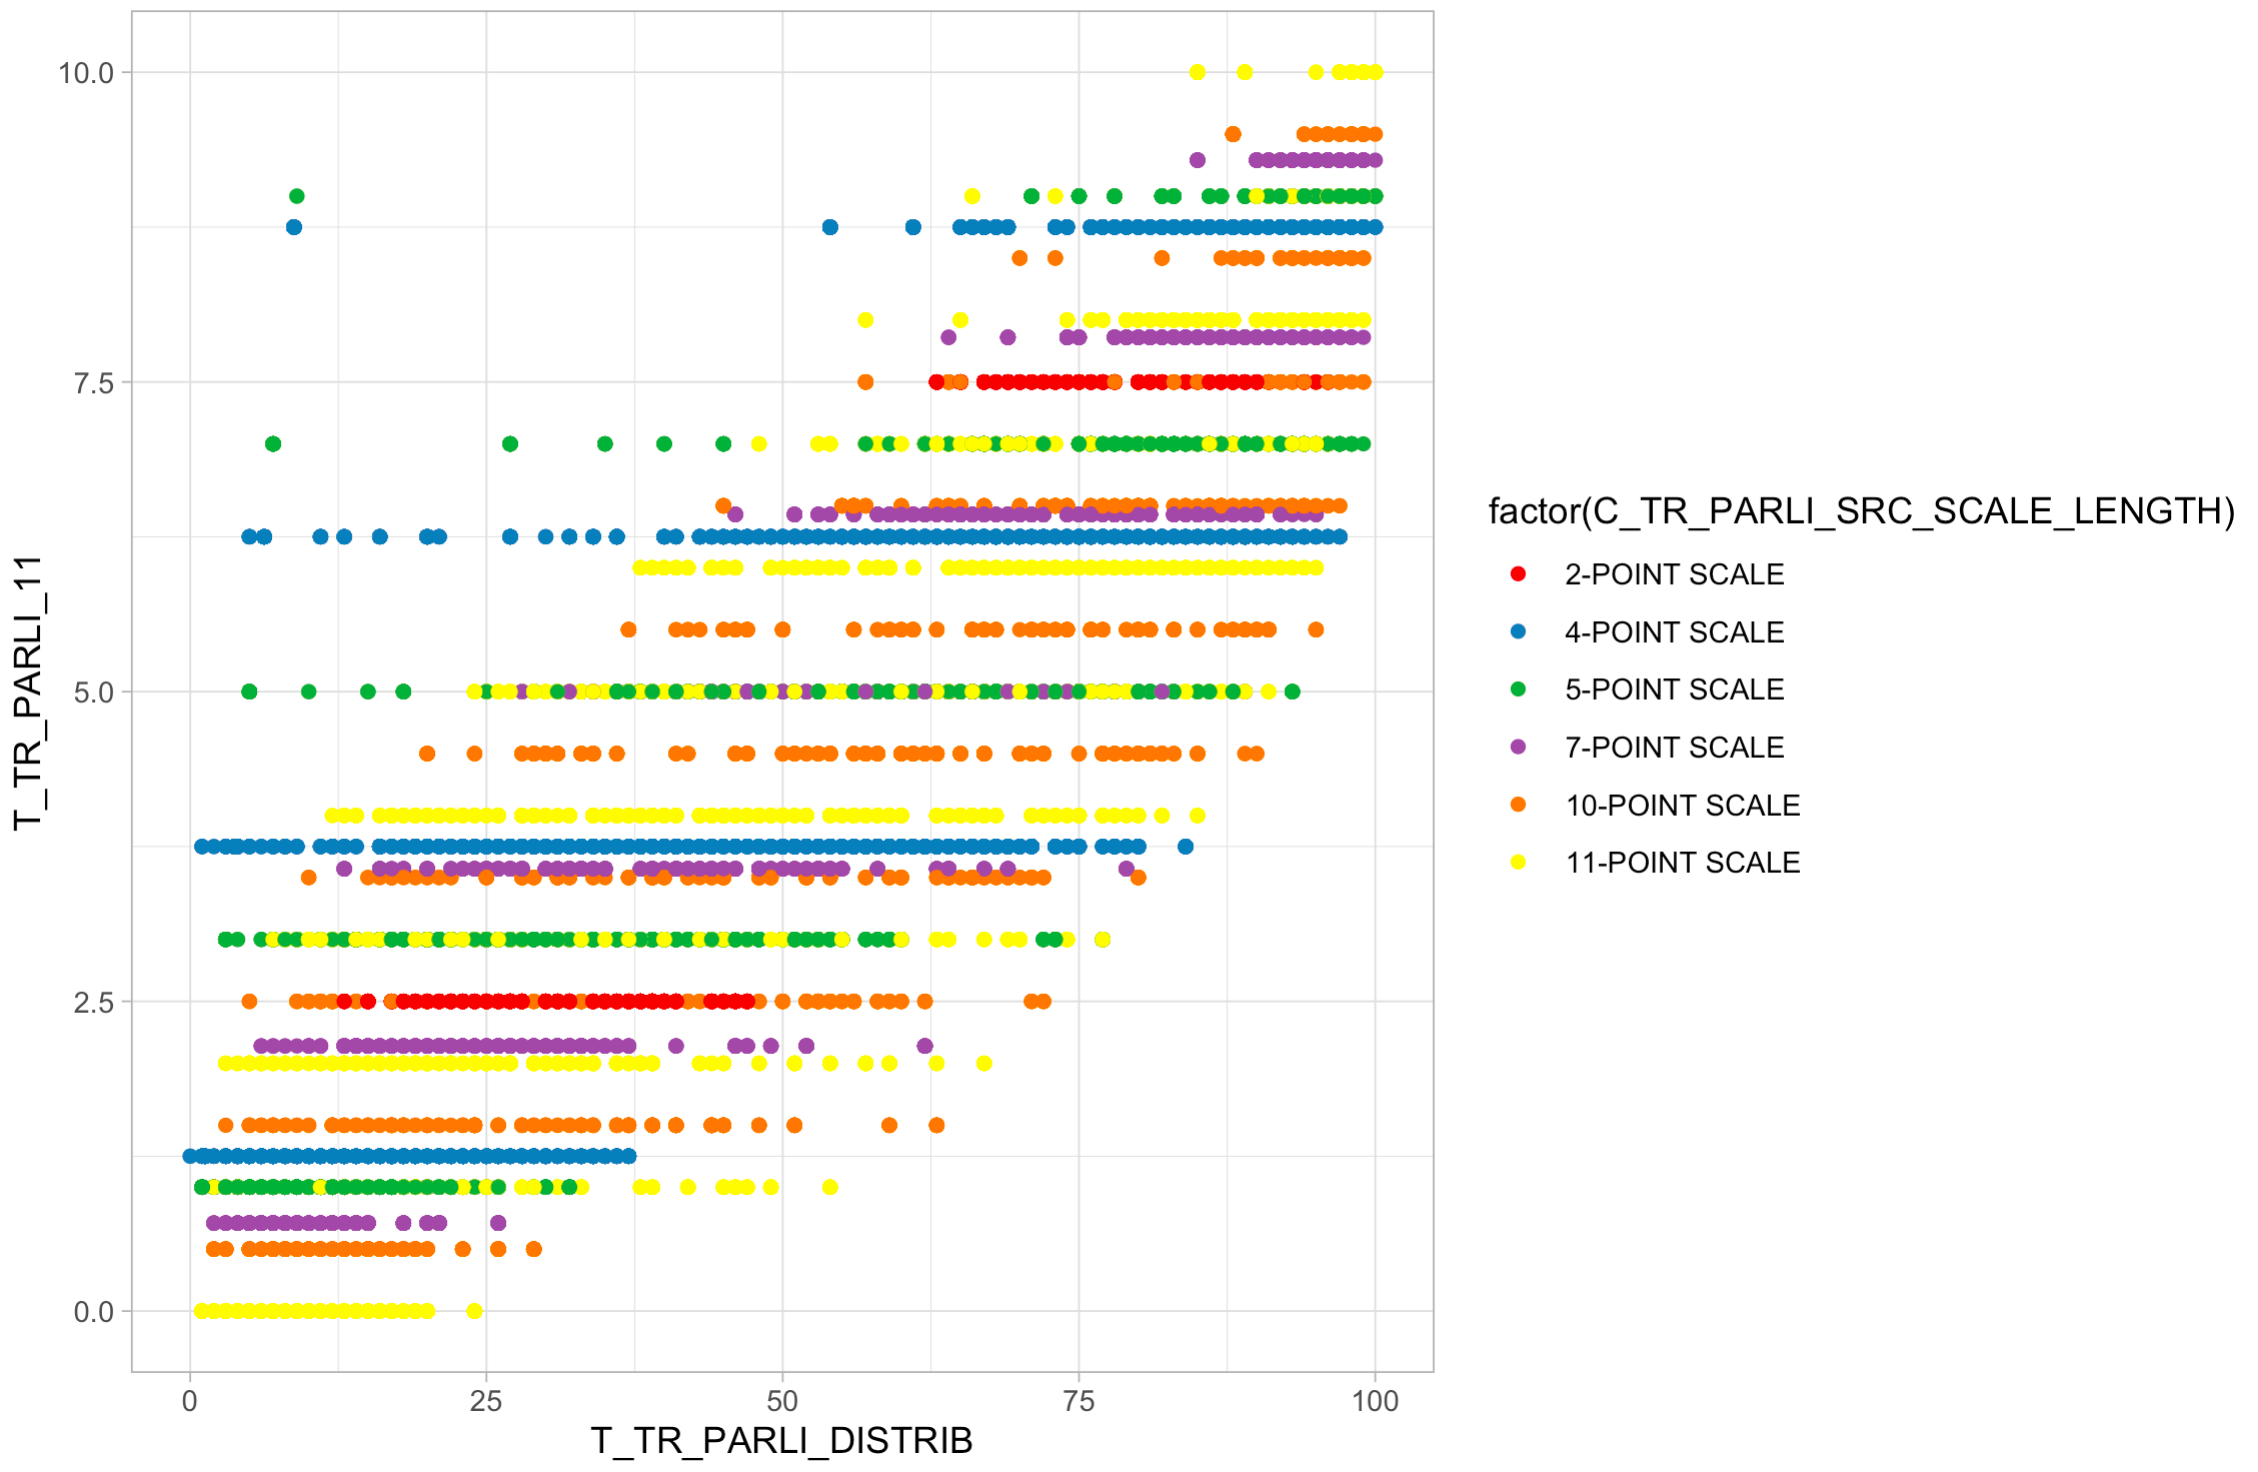
\includegraphics{figures/scatter2.png}

\end{frame}

\begin{frame}{Comments}
\protect\hypertarget{comments}{}

\begin{itemize}
\tightlist
\item
  Untested assumptions

  \begin{itemize}
  \tightlist
  \item
    1/2: equal distance between categories
  \item
    3: same percentile distribution over cohorts
  \end{itemize}
\item
  Arbitrary, not obvious which to choose
\item
  Does not account for response behaviors
\item
  Impact on conclusions
\end{itemize}

\end{frame}

\begin{frame}{Levels of equivalence}
\protect\hypertarget{levels-of-equivalence}{}

\begin{enumerate}
\tightlist
\item
  \textbf{construct inequivalence}: no equivalent concepts across
  cohorts
\item
  \textbf{construct equivalence}: same concept is measured, but scales
  differ
\item
  \textbf{procedural equivalence}: common procedure to measure objects,
  but there is no underlying unit or ordering in the numbers
\item
  \textbf{unit equivalence}: same units but different anchors
\item
  \textbf{scalar equivalence}: same ratio scale across cohort
\end{enumerate}

\end{frame}

\begin{frame}{Idea}
\protect\hypertarget{idea}{}

\begin{itemize}
\tightlist
\item
  Generalize transformation one --\textgreater{} many
\item
  Learn relations from the data
\end{itemize}

\end{frame}

\begin{frame}{Crisp coding}
\protect\hypertarget{crisp-coding}{}

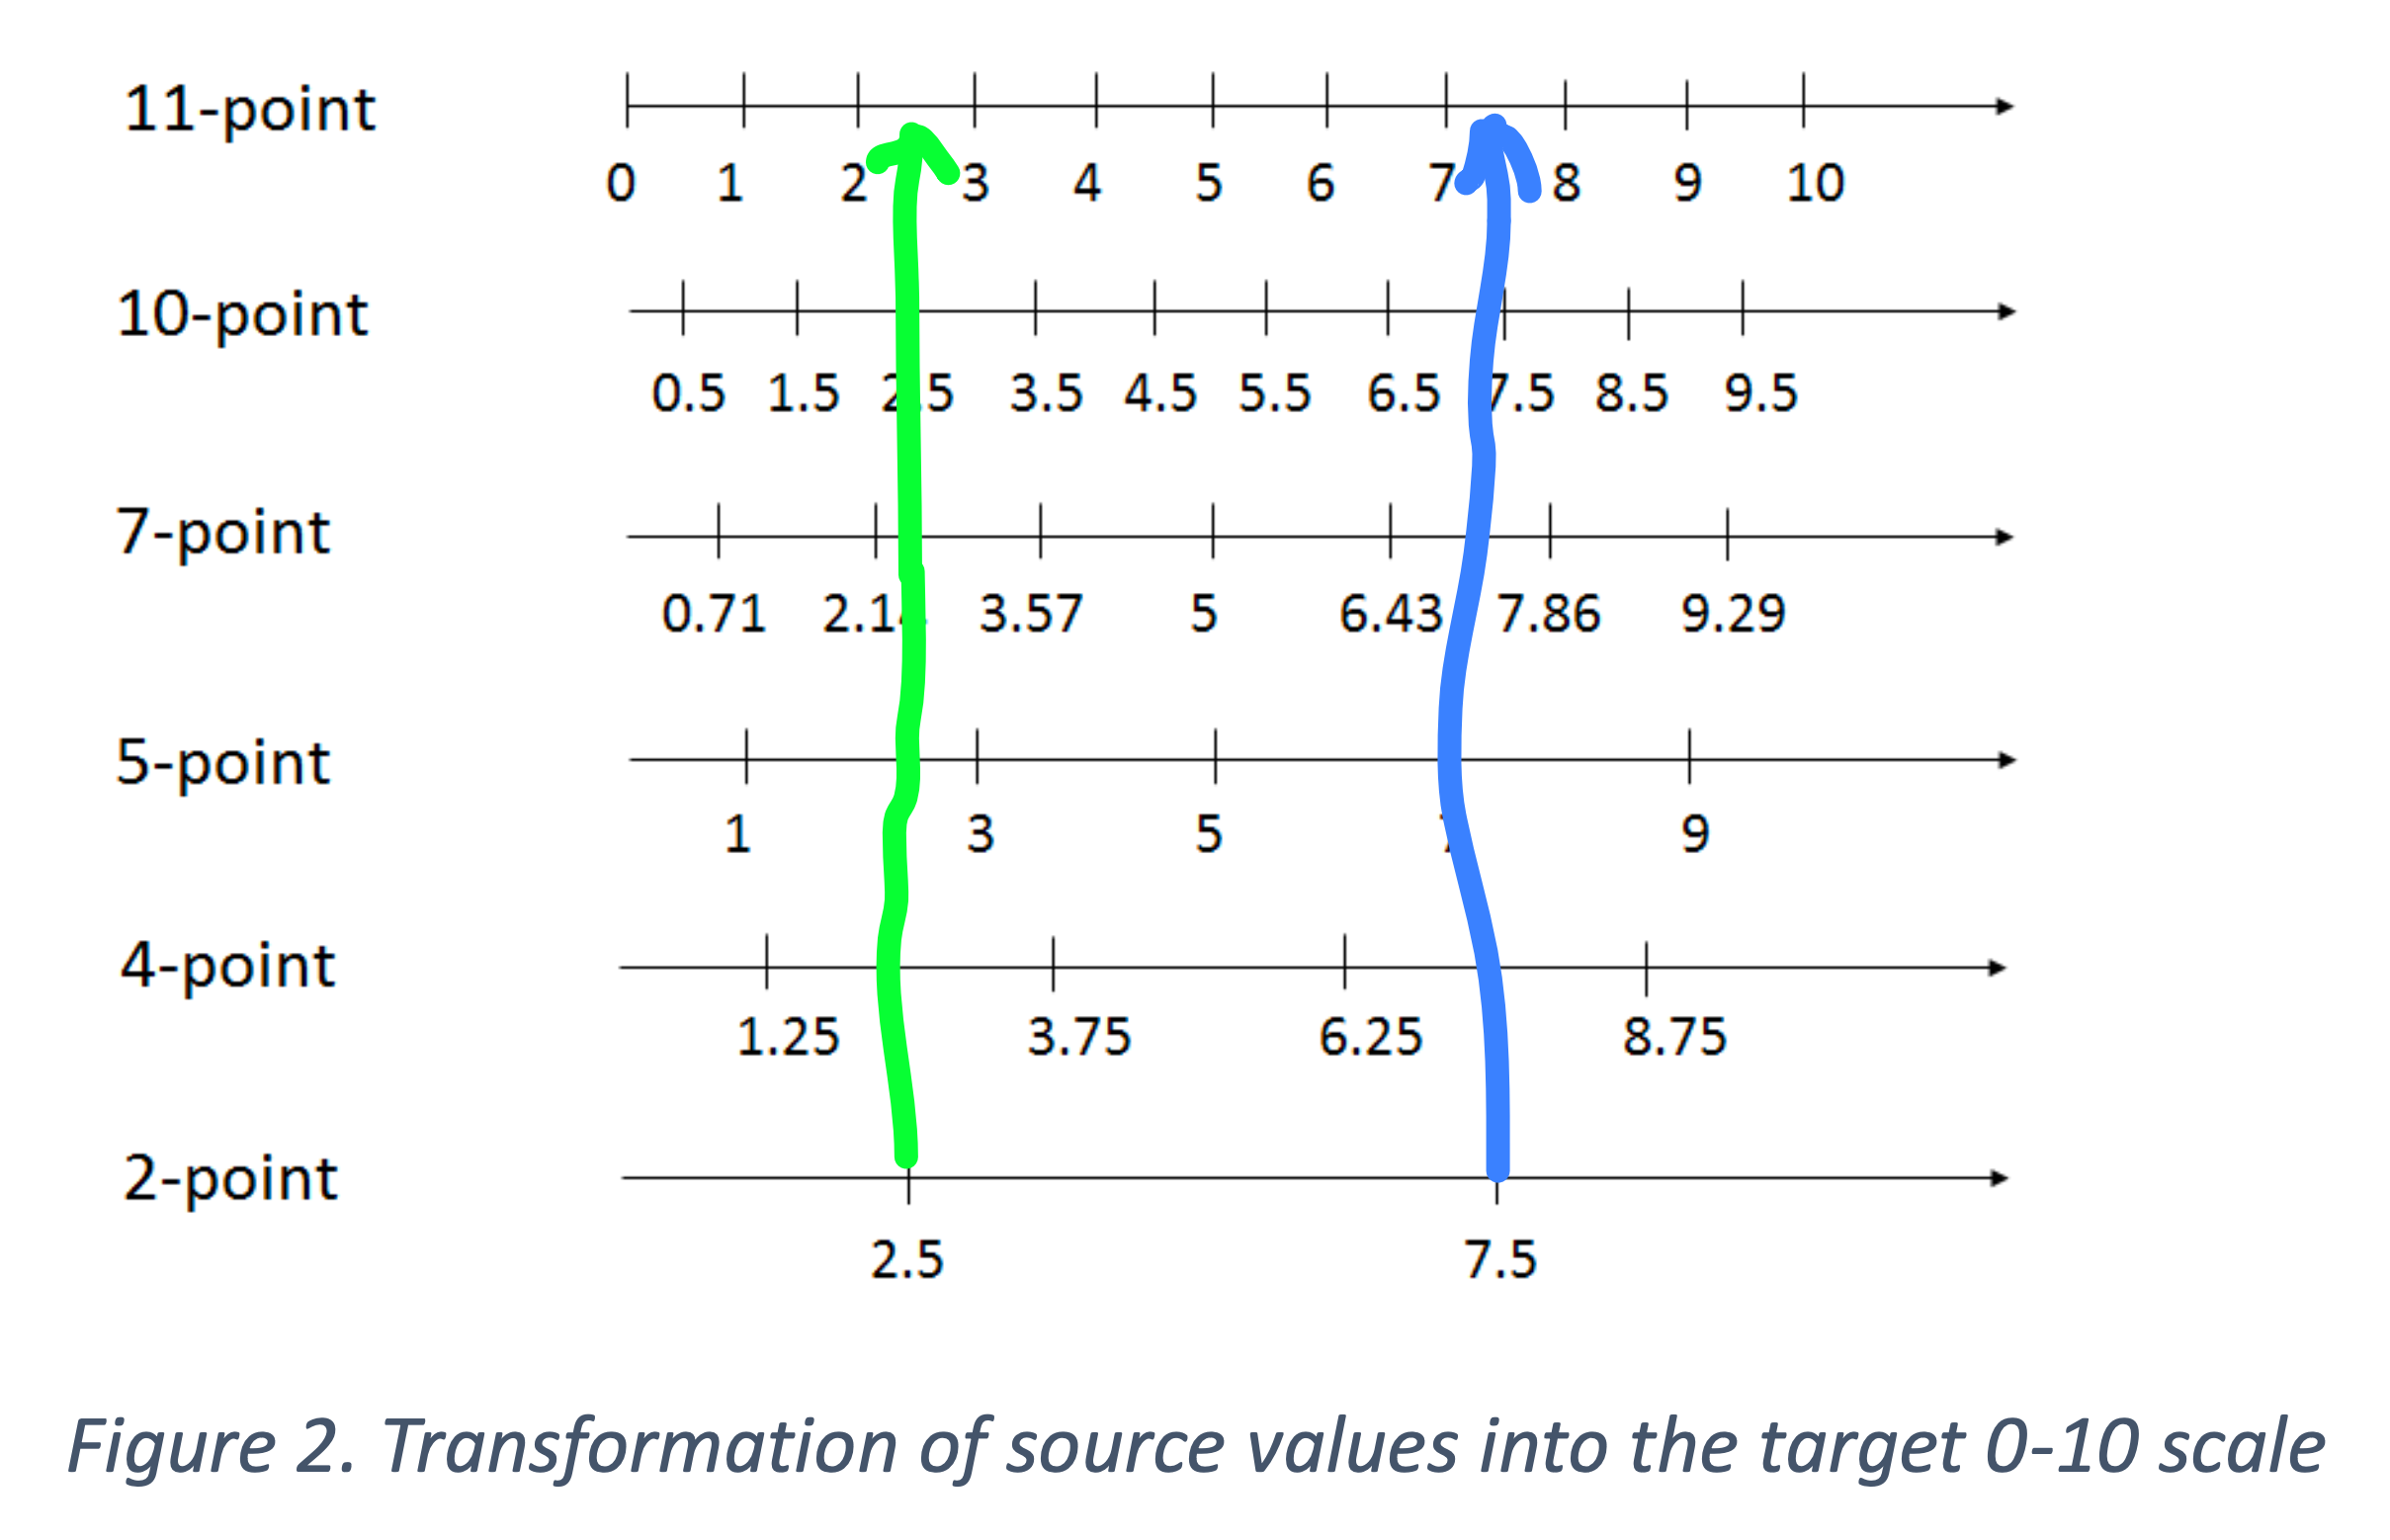
\includegraphics{figures/figure2a.png}

\end{frame}

\begin{frame}{Fuzzy coding}
\protect\hypertarget{fuzzy-coding}{}

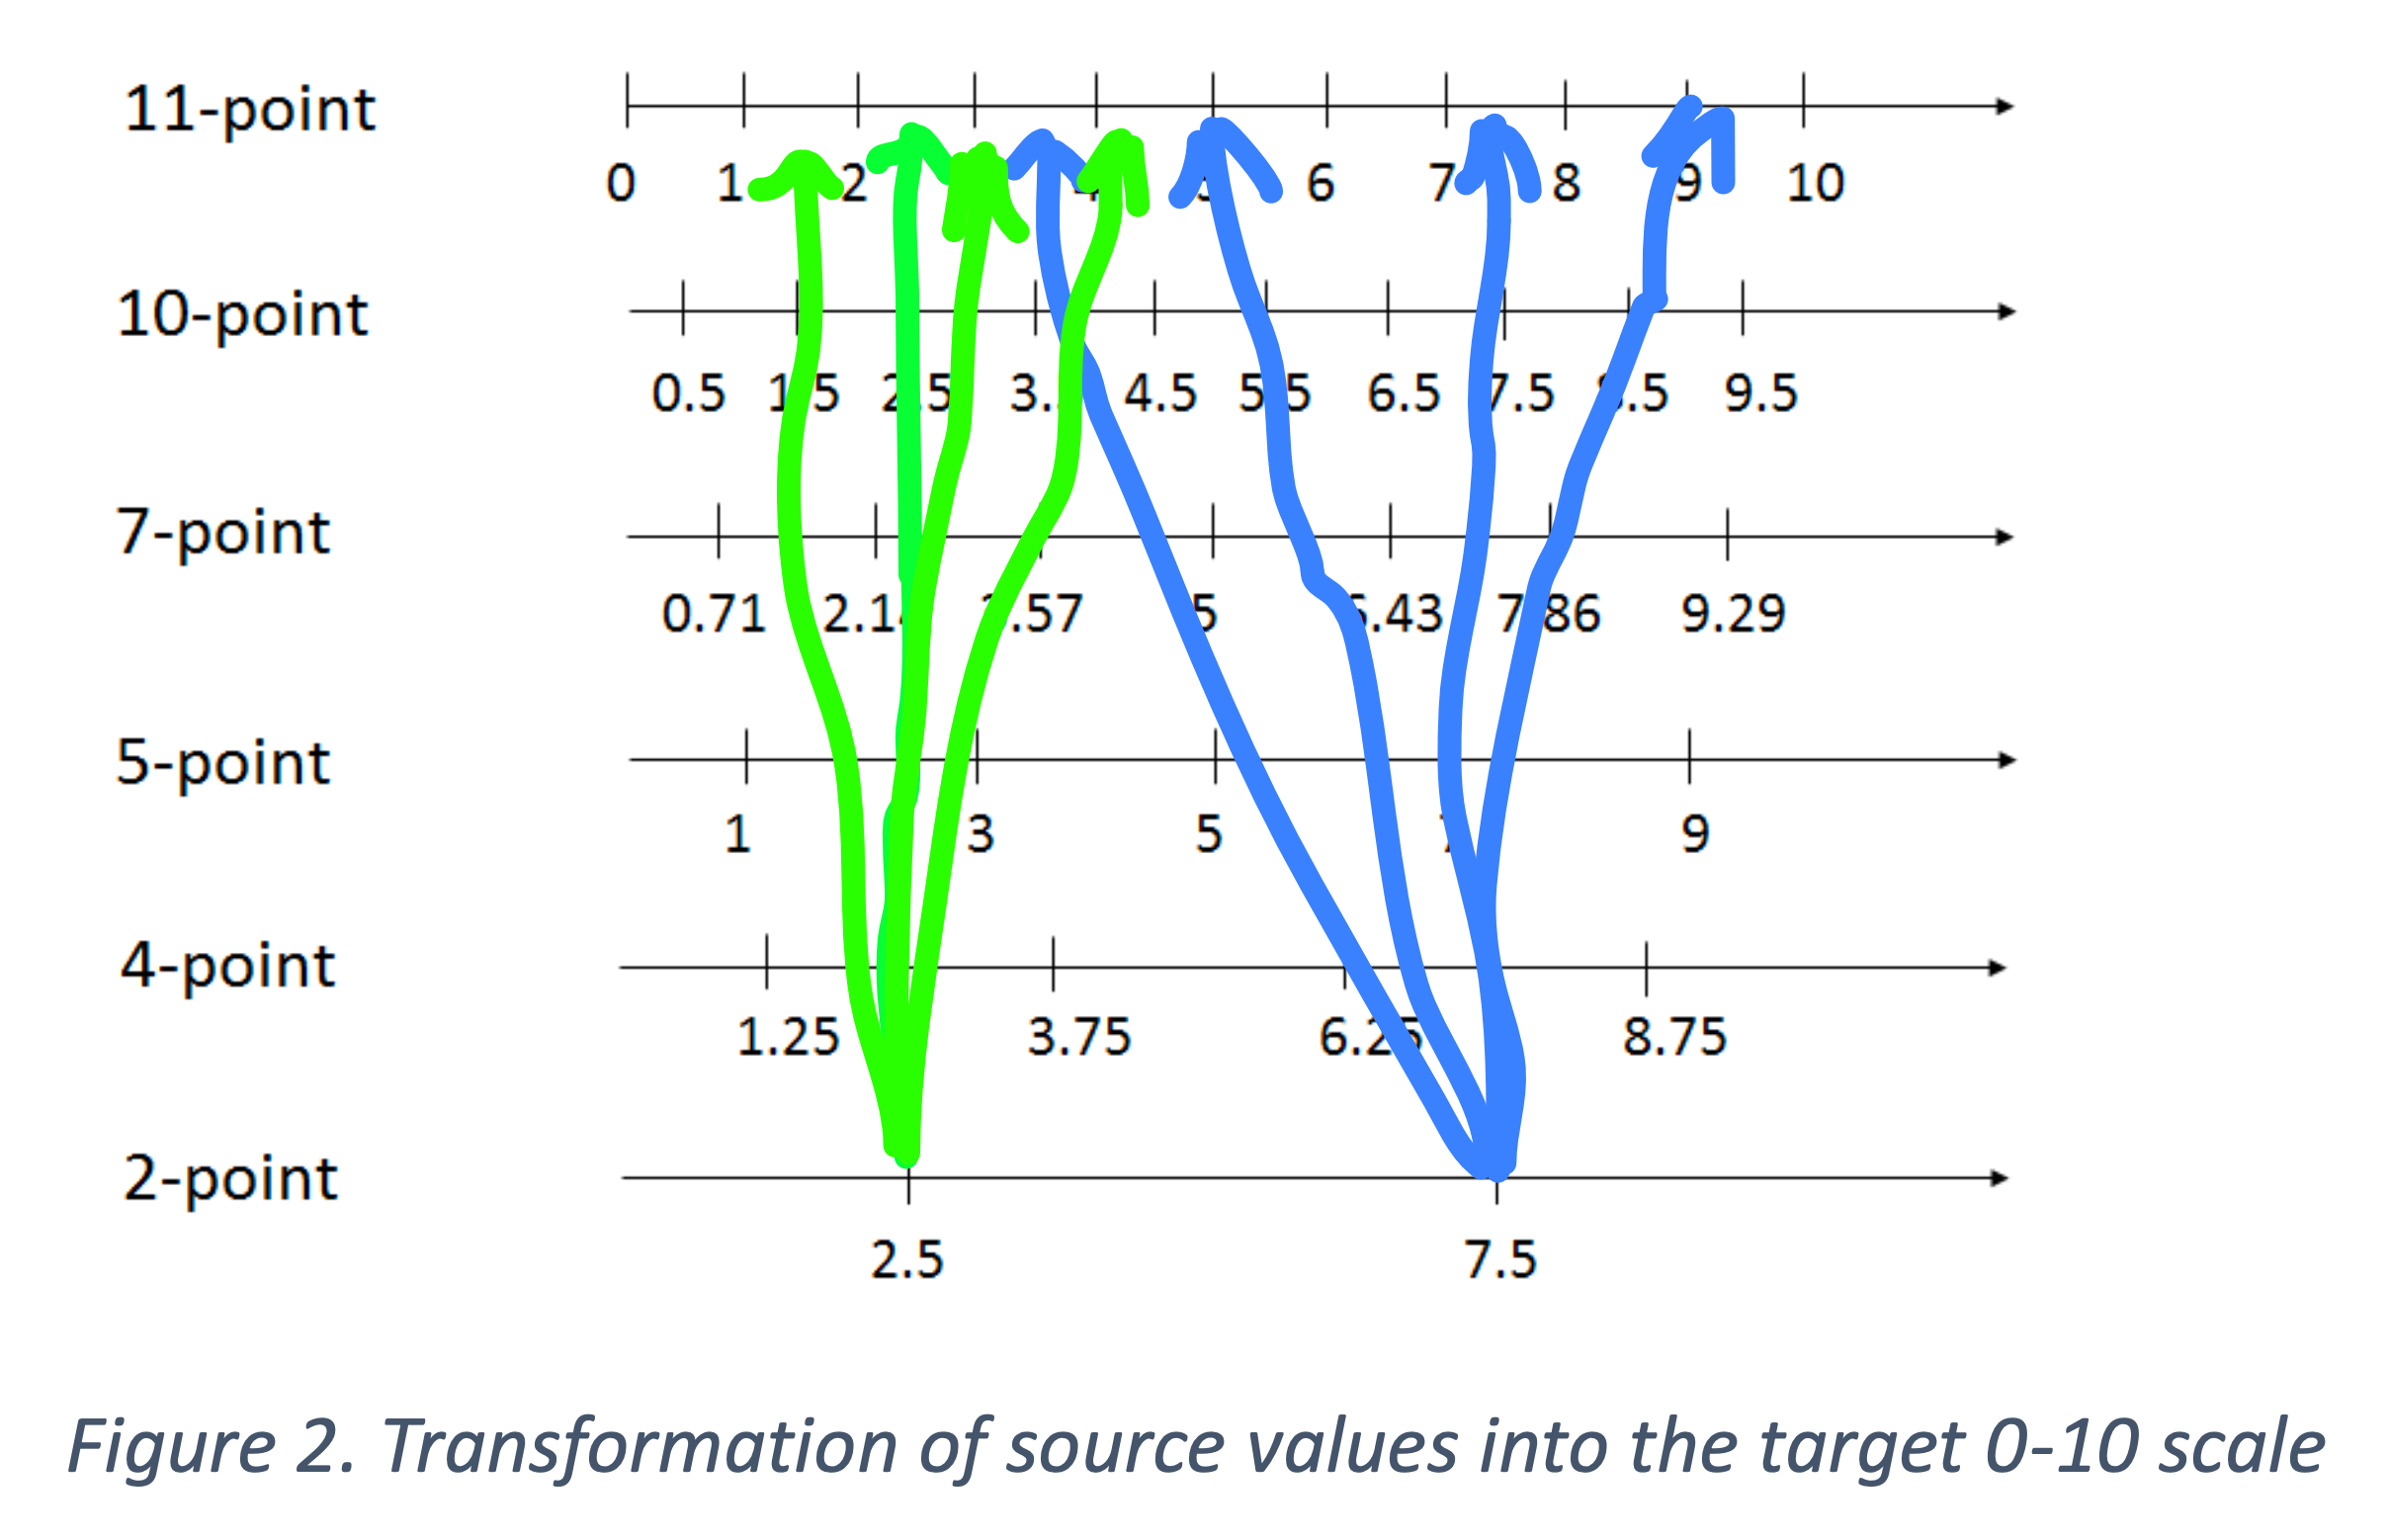
\includegraphics{figures/figure2b.png}

\end{frame}

\begin{frame}{Trust parlement: 0-10 scale, 0-1 scale}
\protect\hypertarget{trust-parlement-0-10-scale-0-1-scale}{}

\begin{longtable}[]{@{}rrrrr@{}}
\toprule
0-10 & no & yes & no & yes\tabularnewline
\midrule
\endhead
0 & 3 & 0 & .02 & .00\tabularnewline
1 & 0 & 0 & .00 & .00\tabularnewline
2 & 6 & 1 & .05 & .01\tabularnewline
3 & 10 & 0 & .08 & .00\tabularnewline
4 & 12 & 1 & .09 & .01\tabularnewline
5 & 30 & 8 & .24 & .05\tabularnewline
6 & 32 & 12 & .25 & .07\tabularnewline
7 & 25 & 54 & .20 & .33\tabularnewline
8 & 8 & 44 & .06 & .27\tabularnewline
9 & 0 & 33 & .00 & .20\tabularnewline
10 & 1 & 8 & .01 & .05\tabularnewline
& & & &\tabularnewline
& 127 & 161 & 1.00 & 1.00\tabularnewline
\bottomrule
\end{longtable}

\end{frame}

\begin{frame}[fragile]{Example: Walking disability in two countries}
\protect\hypertarget{example-walking-disability-in-two-countries}{}

\begin{itemize}
\tightlist
\item
  Uses the \texttt{walking} data in \texttt{mice}
\end{itemize}

\end{frame}

\begin{frame}{Item \texttt{HAQ8} measured in Antonia}
\protect\hypertarget{item-haq8-measured-in-antonia}{}

\textbf{Are you able to walk outdoors on flat ground?}

\begin{longtable}[]{@{}rlr@{}}
\toprule
Cat & Label & Count\tabularnewline
\midrule
\endhead
0 & Without any difficulty & 242\tabularnewline
1 & With some difficulty & 43\tabularnewline
2 & With much difficulty & 15\tabularnewline
3 & Unable to do & 0\tabularnewline
NA & Missing & 6\tabularnewline
& &\tabularnewline
& Total & 306\tabularnewline
\bottomrule
\end{longtable}

Antonia statistic (Mean disability):
\((242 \times 0+43 \times 1+15 \times 2)/ 300 = 0.243\)

\end{frame}

\begin{frame}{Item \texttt{GARS9} measured in Belmark}
\protect\hypertarget{item-gars9-measured-in-belmark}{}

\textbf{Can you, fully independently, walk outdoors (if necessary with a
cane)?}

\begin{longtable}[]{@{}rlr@{}}
\toprule
Cat & Label & Count\tabularnewline
\midrule
\endhead
0 & Yes, no difficulty & 145\tabularnewline
1 & Yes, with some difficulty & 110\tabularnewline
2 & Yes, with much difficulty & 29\tabularnewline
3 & No, only with help from others & 8\tabularnewline
NA & Missing & 0\tabularnewline
& &\tabularnewline
& Total & 292\tabularnewline
\bottomrule
\end{longtable}

Belmark statistic: proportion no difficulty (PND): 145/292 = 0.50

\end{frame}

\begin{frame}{Problem}
\protect\hypertarget{problem}{}

\begin{itemize}
\tightlist
\item
  We want to compare walking problems between Antonia and Belmark
\item
  What to do?
\end{itemize}

\end{frame}

\begin{frame}{The easy way: Equate all categories}
\protect\hypertarget{the-easy-way-equate-all-categories}{}

\begin{longtable}[]{@{}lrr@{}}
\toprule
Country & \emph{Mean} & \emph{PND}\tabularnewline
\midrule
\endhead
Antonia & .24 & .80\tabularnewline
Belmark & .66 & .50\tabularnewline
& &\tabularnewline
Difference & -.42 & .30\tabularnewline
\bottomrule
\end{longtable}

\begin{itemize}
\tightlist
\item
  Both \emph{Mean} and \emph{PND} indicate more walking problems in
  Belmark
\item
  Differences are large
\item
  Assumes that we can perfectly map \emph{HAQ8} into \emph{GARS9}, and
  vice versa.
\item
  That is, the correlation is 1.0: Is that realistic?
\end{itemize}

\end{frame}

\begin{frame}{A third country: Citrus}
\protect\hypertarget{a-third-country-citrus}{}

\begin{longtable}[]{@{}lrrrrlr@{}}
\toprule
& \emph{GARS9 } & & & & &\tabularnewline
\midrule
\endhead
\emph{HAQ8} & 0 & 1 & 2 & 3 & & Total\tabularnewline
& & & & & &\tabularnewline
0 & 256 & 90 & 6 & 4 & & 356\tabularnewline
1 & 26 & 90 & 20 & 0 & & 136\tabularnewline
2 & 6 & 40 & 28 & 10 & & 84\tabularnewline
3 & 0 & 0 & 2 & 2 & & 4\tabularnewline
NA & 2 & 0 & 2 & 0 & & 4\tabularnewline
& & & & & &\tabularnewline
Total & 290 & 220 & 58 & 16 & & 584\tabularnewline
\bottomrule
\end{longtable}

\begin{itemize}
\tightlist
\item
  Not symmetric: \emph{HAQ8} appears more difficult than \emph{GARS9}
\item
  Kendall's \(\tau = 0.57\), not 1.00
\item
  Are there consequences for the comparison?
\end{itemize}

\end{frame}

\begin{frame}{How to impute: data structure}
\protect\hypertarget{how-to-impute-data-structure}{}

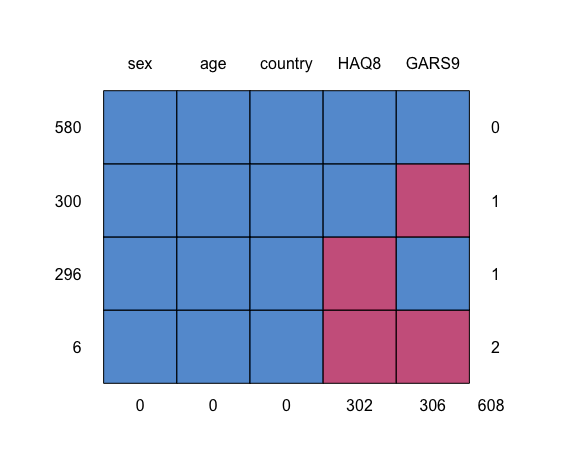
\includegraphics{figures/mdpattern.png}

\end{frame}

\begin{frame}{How to impute: Kendall's \(\tau\) for imputed HAQ8 and
GARS9}
\protect\hypertarget{how-to-impute-kendalls-tau-for-imputed-haq8-and-gars9}{}

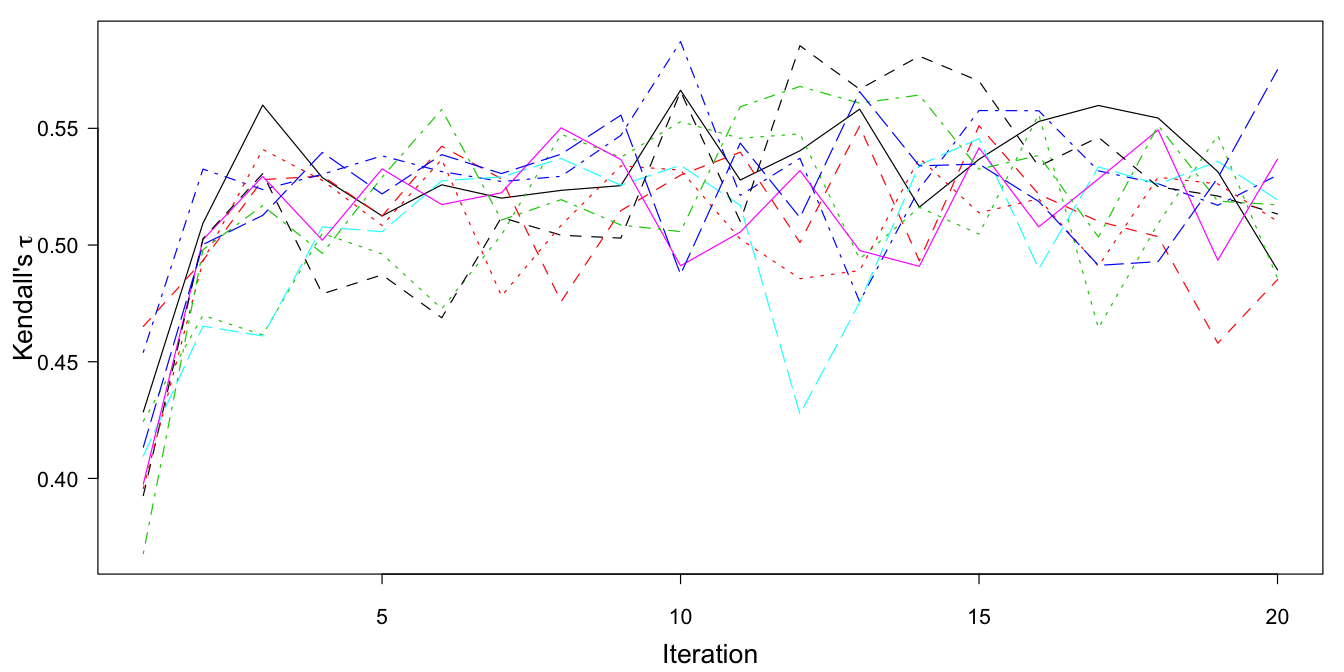
\includegraphics{figures/ch9-walkingimpute7b-1.png}

\end{frame}

\begin{frame}{Result: Proportion No difficulty (\emph{PND}) in Antonia}
\protect\hypertarget{result-proportion-no-difficulty-pnd-in-antonia}{}

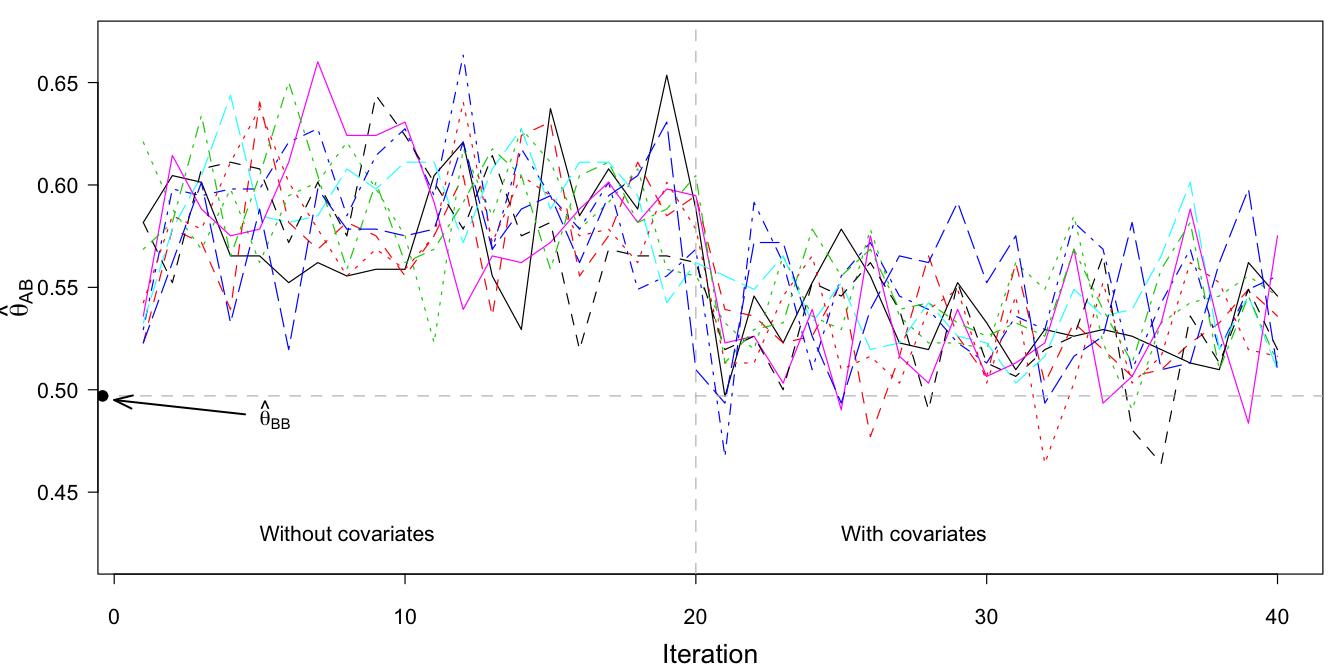
\includegraphics{figures/ch9-walkingplotthetaAB-1.png}

\end{frame}

\begin{frame}{Results: equating \textless{}--\textgreater{} MI
\textless{}--\textgreater{} MI + age + sex}
\protect\hypertarget{results-equating-mi-mi-age-sex}{}

\begin{longtable}[]{@{}lrrrrrrrr@{}}
\toprule
Country & \emph{Mean} & \emph{PND} & & \emph{Mean} & \emph{PND} & &
\emph{Mean} & \emph{PND}\tabularnewline
\midrule
\endhead
Antonia & .24 & .80 & & .24 & .59 & & .24 & .53\tabularnewline
Belmark & .66 & .50 & & .45 & .50 & & .45 & .50\tabularnewline
& & & & & & & &\tabularnewline
Difference & -.42 & .30 & & -.22 & .09 & & -.22 & .03\tabularnewline
\bottomrule
\end{longtable}

\begin{itemize}
\tightlist
\item
  Antonia is still doing better, but the effects are much smaller
\item
  Correction has more effect on ``proportion of no difficulty''
  (\emph{PND}) (10 times smaller!)
\end{itemize}

\end{frame}

\begin{frame}{Conclusions}
\protect\hypertarget{conclusions}{}

\begin{itemize}
\item
  \textbf{Simple equating exaggerates differences between countries},
  e.g., +30 percent points instead of +3 percent points
\item
  Overstated differences may spur inappropriate interventions, sometimes
  with substantial financial consequences
\item
  Worse problems exist for the different number of categories, popular
  \emph{crisp recoding}
\item
  Advised remedy: multiple imputation, including covariates
\item
  More detail:
  \url{https://stefvanbuuren.name/fimd/sec-codingsystems.html}
\item
  Code:
  \url{https://github.com/stefvanbuuren/fimdbook/blob/master/R/fimd.R}
\end{itemize}

\end{frame}

\begin{frame}{2. Uncollected variables}
\protect\hypertarget{uncollected-variables}{}

Analysis of individual patient data (IPD) is very popular. It has many
advantages over meta-analysis of aggregate data, e.g.,

\begin{itemize}
\tightlist
\item
  Consistent inclusion/exclusion criteria
\item
  Missing data can be treated at the patient level
\item
  Verifies original analysis
\item
  Removal of duplicate subjects
\item
  Consistent correction for confounders
\end{itemize}

\end{frame}

\begin{frame}{Problem: Studies collect different variables}
\protect\hypertarget{problem-studies-collect-different-variables}{}

Missing data in IPD

\begin{itemize}
\item
  \textbf{Systematically missing}: Not collected, missing for all in
  study
\item
  \textbf{Sporadically missing}: Collected, but missing for some in
  study
\item
  Can be at level-1 or level-2 of the analysis
\end{itemize}

\end{frame}

\begin{frame}[fragile]{Imputation of IPD data}
\protect\hypertarget{imputation-of-ipd-data}{}

\begin{itemize}
\tightlist
\item
  In general, we need multilevel imputation models
\item
  Historically, most techniques were suited only for sporadically
  missing
\item
  Wish to preserve between-study heterogeneity in errors:
  \texttt{mice::mice.impute.2l.norm()}
\item
  More recently, two types of models, level-1:

  \begin{itemize}
  \tightlist
  \item
    generalization to systematically missing:
    \texttt{mice::mice.impute.2l.lmer()} (Jolani, 2016)
  \item
    2-stage models: \texttt{micemd::mice.impute.2l.2stage.norm()}
    (Resche-Rigon 2016)
  \end{itemize}
\end{itemize}

\end{frame}

\begin{frame}[fragile]{\texttt{brandsma} data}
\protect\hypertarget{brandsma-data}{}

\begin{itemize}
\tightlist
\item
  Brandsma and Knuver, Int J Ed Res, 1989.
\item
  Extensively discussed in Snijders and Bosker (2012), 2nd ed.
\item
  4106 pupils, 216 schools, about 4\% missing values
\end{itemize}

\begin{Shaded}
\begin{Highlighting}[]
\KeywordTok{library}\NormalTok{(mice)}
\KeywordTok{head}\NormalTok{(brandsma[, }\KeywordTok{c}\NormalTok{(}\DecValTok{1}\OperatorTok{:}\DecValTok{6}\NormalTok{, }\DecValTok{9}\OperatorTok{:}\DecValTok{10}\NormalTok{, }\DecValTok{13}\NormalTok{)], }\DecValTok{3}\NormalTok{)}
\end{Highlighting}
\end{Shaded}

\begin{verbatim}
##   sch pup   iqv   iqp sex    ses lpr lpo den
## 1   1   1 -1.35 -3.72   1 -17.67  33  NA   1
## 2   1   2  2.15  3.28   1     NA  44  50   1
## 3   1   3  3.15  1.27   0  -4.67  36  46   1
\end{verbatim}

\end{frame}

\begin{frame}[fragile]{\texttt{brandsma} data subset}
\protect\hypertarget{brandsma-data-subset}{}

\begin{Shaded}
\begin{Highlighting}[]
\NormalTok{d <-}\StringTok{ }\NormalTok{brandsma[, }\KeywordTok{c}\NormalTok{(}\StringTok{"sch"}\NormalTok{, }\StringTok{"lpo"}\NormalTok{, }\StringTok{"sex"}\NormalTok{, }\StringTok{"den"}\NormalTok{)]}
\KeywordTok{head}\NormalTok{(d, }\DecValTok{2}\NormalTok{)}
\end{Highlighting}
\end{Shaded}

\begin{verbatim}
##   sch lpo sex den
## 1   1  NA   1   1
## 2   1  50   1   1
\end{verbatim}

\begin{itemize}
\tightlist
\item
  \texttt{sch}: School number, cluster variable, \(C = 216\);
\item
  \texttt{lpo}: Language test post, outcome at pupil level;
\item
  \texttt{sex}: Sex of pupil, predictor at pupil level (0-1);
\item
  \texttt{den}: School denomination, predictor at school level (1-4).
\end{itemize}

\end{frame}

\begin{frame}[fragile]{Model of scientific interest}
\protect\hypertarget{model-of-scientific-interest}{}

Predict \texttt{lpo} from the

\begin{itemize}
\tightlist
\item
  level-1 predictor \texttt{sex}
\item
  level-2 predictor \texttt{den}
\end{itemize}

\end{frame}

\begin{frame}{Level notation - Bryk and Raudenbush (1992)}
\protect\hypertarget{level-notation---bryk-and-raudenbush-1992}{}

\begin{align}
{{\texttt{lpo}}}_{ic} & = \beta_{0c} + \beta_{1c}{{\texttt{sex}}}_{ic} + \epsilon_{ic}\\
\beta_{0c}     & = \gamma_{00} + \gamma_{01}{{\texttt{den}}}_{c} + u_{0c}\\
\beta_{1c}     & = \gamma_{10}
\end{align}

\begin{itemize}
\tightlist
\item
  \(\text{lpo}_{ic}\) is the test score of pupil \(i\) in school \(c\)
\item
  \(\text{sex}_{ic}\) is the sex of pupil \(i\) in school \(c\)
\item
  \(\text{den}_c\) is the religious denomination of school \(c\)
\item
  \(\beta_{0c}\) is a random intercept that varies by cluster
\item
  \(\beta_{1c}\) is a sex effect, assumed to be the same across schools.
\item
  \(\epsilon_{ic} \sim N(0, \sigma_\epsilon^2)\) is the within-cluster
  random residual at the pupil level
\end{itemize}

\end{frame}

\begin{frame}{Level 2 equations: interpretation}
\protect\hypertarget{level-2-equations-interpretation}{}

The first level-2 model
\[\beta_{0c} = \gamma_{00} + \gamma_{01}\text{den}_c + u_{0c}, \]
describes the variation in the mean test score between schools as a
function of

\begin{itemize}
\tightlist
\item
  the grand mean \(\gamma_{00}\),
\item
  a school-level effect \(\gamma_{01}\) of denomination, and a
\item
  school-level random residual \(u_{0c}\sim N(0, \sigma_{u_0}^2)\)
\end{itemize}

The second level 2 model \[\beta_{1c} = \gamma_{10},\] specifies
\(\beta_{1c}\) as a fixed effect equal in value to \(\gamma_{10}\)

\end{frame}

\begin{frame}{Unknown parameters}
\protect\hypertarget{unknown-parameters}{}

\begin{align}
{{\texttt{lpo}}}_{ic} & = \beta_{0c} + \beta_{1c}{{\texttt{sex}}}_{ic} + \epsilon_{ic}\\
\beta_{0c}     & = \gamma_{00} + \gamma_{01}{{\texttt{den}}}_{c} + u_{0c}\\
\beta_{1c}     & = \gamma_{10}
\end{align}

The unknowns to be estimated are the fixed parameters:

\begin{itemize}
\tightlist
\item
  \(\gamma_{00}\),
\item
  \(\gamma_{01}\), and
\item
  \(\gamma_{10},\)
\end{itemize}

and the variance components:

\begin{itemize}
\tightlist
\item
  \(\sigma_\epsilon^2\) and
\item
  \(\sigma_{u_0}^2.\)
\end{itemize}

\end{frame}

\begin{frame}{Where are the missings?}
\protect\hypertarget{where-are-the-missings}{}

In single level data, missingness may be in the outcome and/or in the
predictors

With multilevel data, missingness may be in:

\begin{enumerate}
\item
  the outcome variable;
\item
  the level-1 predictors;
\item
  the level-2 predictors;
\item
  the class variable.
\end{enumerate}

\end{frame}

\begin{frame}{Univariate missing, level-1 outcome}
\protect\hypertarget{univariate-missing-level-1-outcome}{}

\begin{center}\includegraphics[height=3in]{Lecture_2_files/figure-beamer/unnamed-chunk-14-1} \end{center}

\end{frame}

\begin{frame}{Univariate missing, level-1 predictor, sporadically
missing}
\protect\hypertarget{univariate-missing-level-1-predictor-sporadically-missing}{}

\begin{center}\includegraphics[height=3in]{Lecture_2_files/figure-beamer/unnamed-chunk-15-1} \end{center}

\end{frame}

\begin{frame}{Univariate missing, level-1 predictor, systematically
missing}
\protect\hypertarget{univariate-missing-level-1-predictor-systematically-missing}{}

\begin{center}\includegraphics[height=3in]{Lecture_2_files/figure-beamer/unnamed-chunk-16-1} \end{center}

\end{frame}

\begin{frame}{Univariate missing, level-2 predictor}
\protect\hypertarget{univariate-missing-level-2-predictor}{}

\begin{center}\includegraphics[height=3in]{Lecture_2_files/figure-beamer/unnamed-chunk-17-1} \end{center}

\end{frame}

\begin{frame}{Multivariate missing}
\protect\hypertarget{multivariate-missing}{}

\begin{center}\includegraphics[height=3in]{Lecture_2_files/figure-beamer/unnamed-chunk-18-1} \end{center}

\end{frame}

\begin{frame}{Nine challenges in multilevel imputation (1 of 3)}
\protect\hypertarget{nine-challenges-in-multilevel-imputation-1-of-3}{}

\begin{enumerate}
\item
  For small clusters the within-cluster mean and variance are unreliable
  estimates, so the choice of the prior distribution becomes critical.
\item
  For a small number of clusters, it is difficult to estimate the
  between-cluster variance of the random effects.
\item
  In applications with systematically missing data, there are no
  observed values in the cluster, so the cluster location cannot be
  estimated.
\end{enumerate}

\end{frame}

\begin{frame}{Nine challenges in multilevel imputation (2 of 3)}
\protect\hypertarget{nine-challenges-in-multilevel-imputation-2-of-3}{}

\begin{enumerate}
\setcounter{enumi}{3}
\item
  The variation of the random slopes can be large, and some methods have
  difficulty handling this.
\item
  The error variance \(\sigma_\epsilon^2\) may differ across clusters
  (heteroscedasticity), whereas the standard model assumes equal error
  variances.
\item
  The residual error distributions can be far from normal, e.g., for
  categorical data.
\end{enumerate}

\end{frame}

\begin{frame}{Nine challenges in multilevel imputation (3 of 3)}
\protect\hypertarget{nine-challenges-in-multilevel-imputation-3-of-3}{}

\begin{enumerate}
\setcounter{enumi}{6}
\item
  The model may contain aggregates of the level-1 variables, such as
  cluster means, which need to be taken in account during imputation.
\item
  The model may contain interactions, or other nonlinear terms.
\item
  It may not be possible to fit the multilevel model, or there are
  convergence problems.
\end{enumerate}

See \href{https://stefvanbuuren.name/fimd/sec-missmult.html}{Van Buuren
(2018)}

\end{frame}

\begin{frame}{Ad hoc solutions}
\protect\hypertarget{ad-hoc-solutions}{}

\begin{enumerate}
\tightlist
\item
  Listwise deletion: Generally not recommended
\item
  Single-level imputation: Biases ICC downwards.
\end{enumerate}

\begin{itemize}
\tightlist
\item
  Conducting multiple imputation with the wrong model (e.g.,
  single-level methods) can be more hazardous than listwise deletion.
\end{itemize}

\begin{enumerate}
\setcounter{enumi}{2}
\tightlist
\item
  Include dummy per cluster: Fixed effects generally unbiased, but the
  random effects are not. Biases ICC upwards.
\end{enumerate}

\end{frame}

\begin{frame}{Three general strategies}
\protect\hypertarget{three-general-strategies}{}

\begin{itemize}
\tightlist
\item
  Monotone data imputation
\item
  Joint modeling
\item
  Fully conditional specification (FCS)
\end{itemize}

\end{frame}

\begin{frame}{Fully conditional specification}
\protect\hypertarget{fully-conditional-specification}{}

\begin{align}
\dot{{\texttt{lpo}}}_{ic} & \sim N(\beta_0 + \beta_1 {{\texttt{den}}}_{c} + \beta_2 {{\texttt{sex}}}_{ic} + u_{0c}, \sigma_\epsilon^2)\\
\dot{{\texttt{sex}}}_{ic} & \sim N(\beta_0 + \beta_1 {{\texttt{den}}}_{c} + \beta_2 {{\texttt{lpo}}}_{ic} + u_{0c}, \sigma_\epsilon^2)
\end{align}

\end{frame}

\begin{frame}{Theoretical problem with FCS}
\protect\hypertarget{theoretical-problem-with-fcs}{}

Conditional expectation of \(\texttt{sex}_{ic}\) in a random effects
model depends on

\begin{itemize}
\tightlist
\item
  \(\texttt{lpo}_{ic}\),
\item
  \(\overline{\texttt{lpo}}_{i}\), the mean of cluster \(i\), and
\item
  \(n_i\), the size of cluster \(i\).
\end{itemize}

Resche-Rigon \& White (2018) suggest the imputation model

\begin{itemize}
\tightlist
\item
  should incorporate the cluster means of level-1 predictors
\item
  be heteroscedastic if cluster sizes vary
\end{itemize}

\end{frame}

\begin{frame}{Methods for multilevel imputation in \texttt{mice}}
\protect\hypertarget{methods-for-multilevel-imputation-in-mice}{}

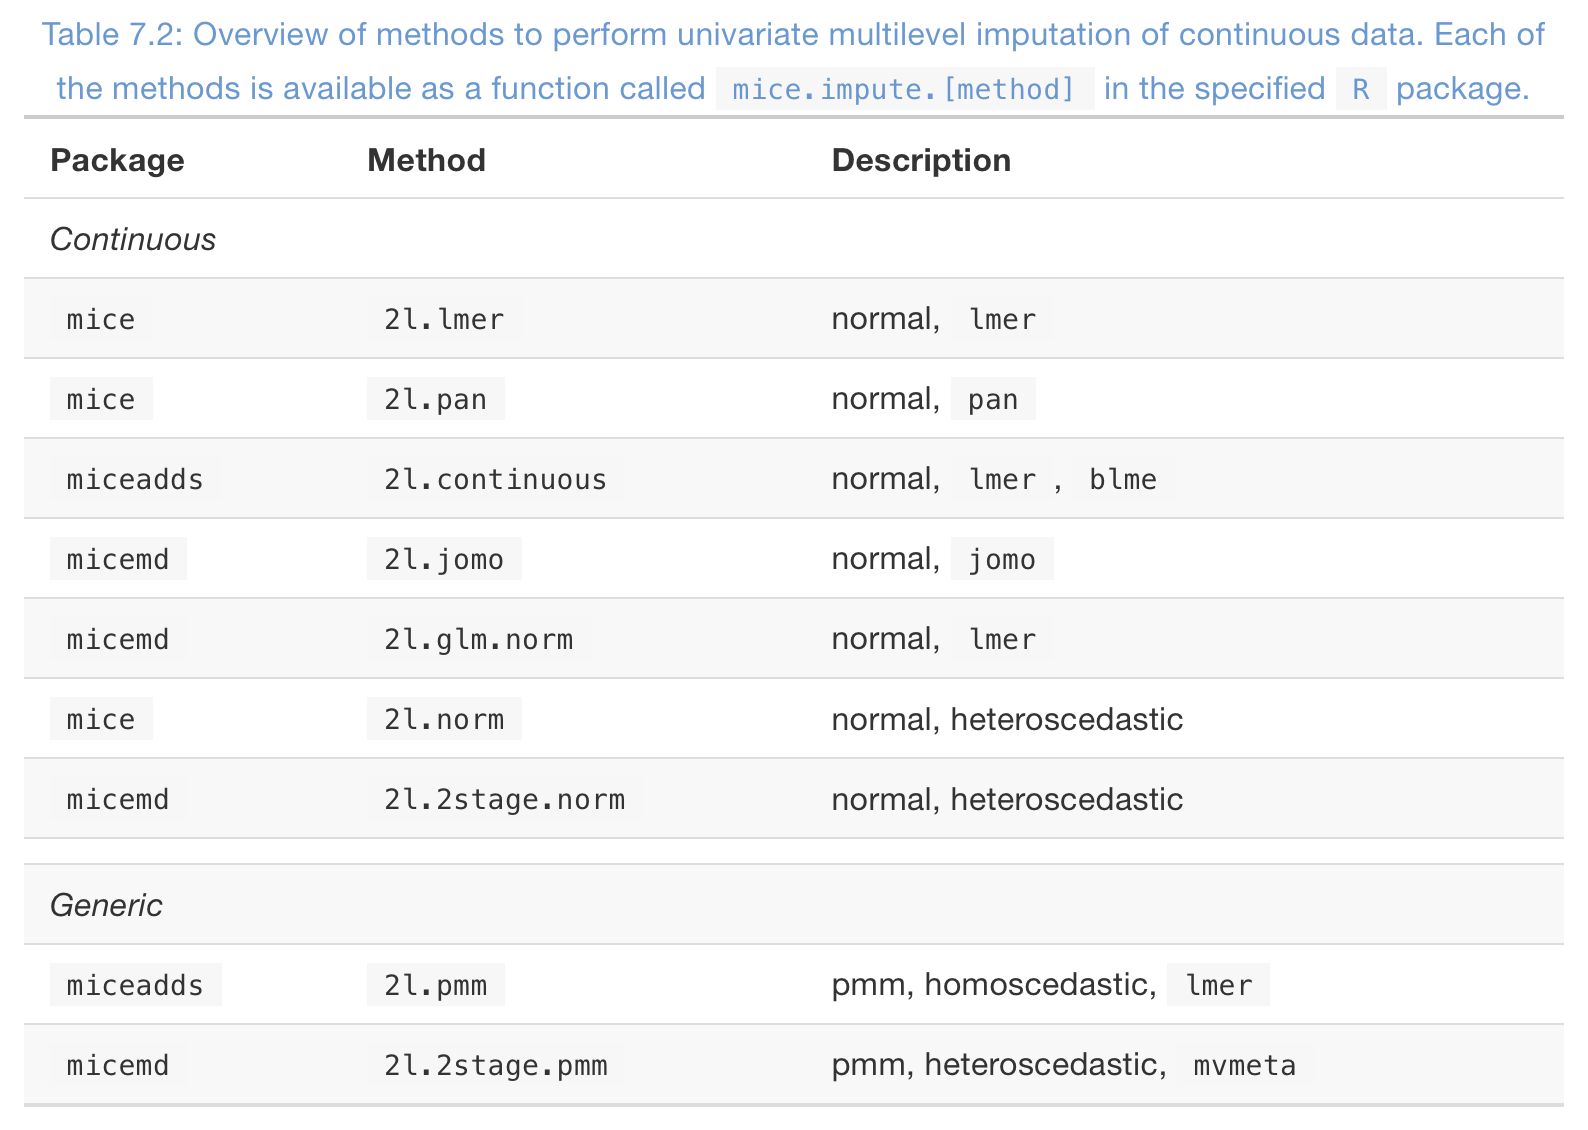
\includegraphics{figures/fig1.png}

\end{frame}

\begin{frame}{Methods for multilevel imputation in \texttt{mice}}
\protect\hypertarget{methods-for-multilevel-imputation-in-mice-1}{}

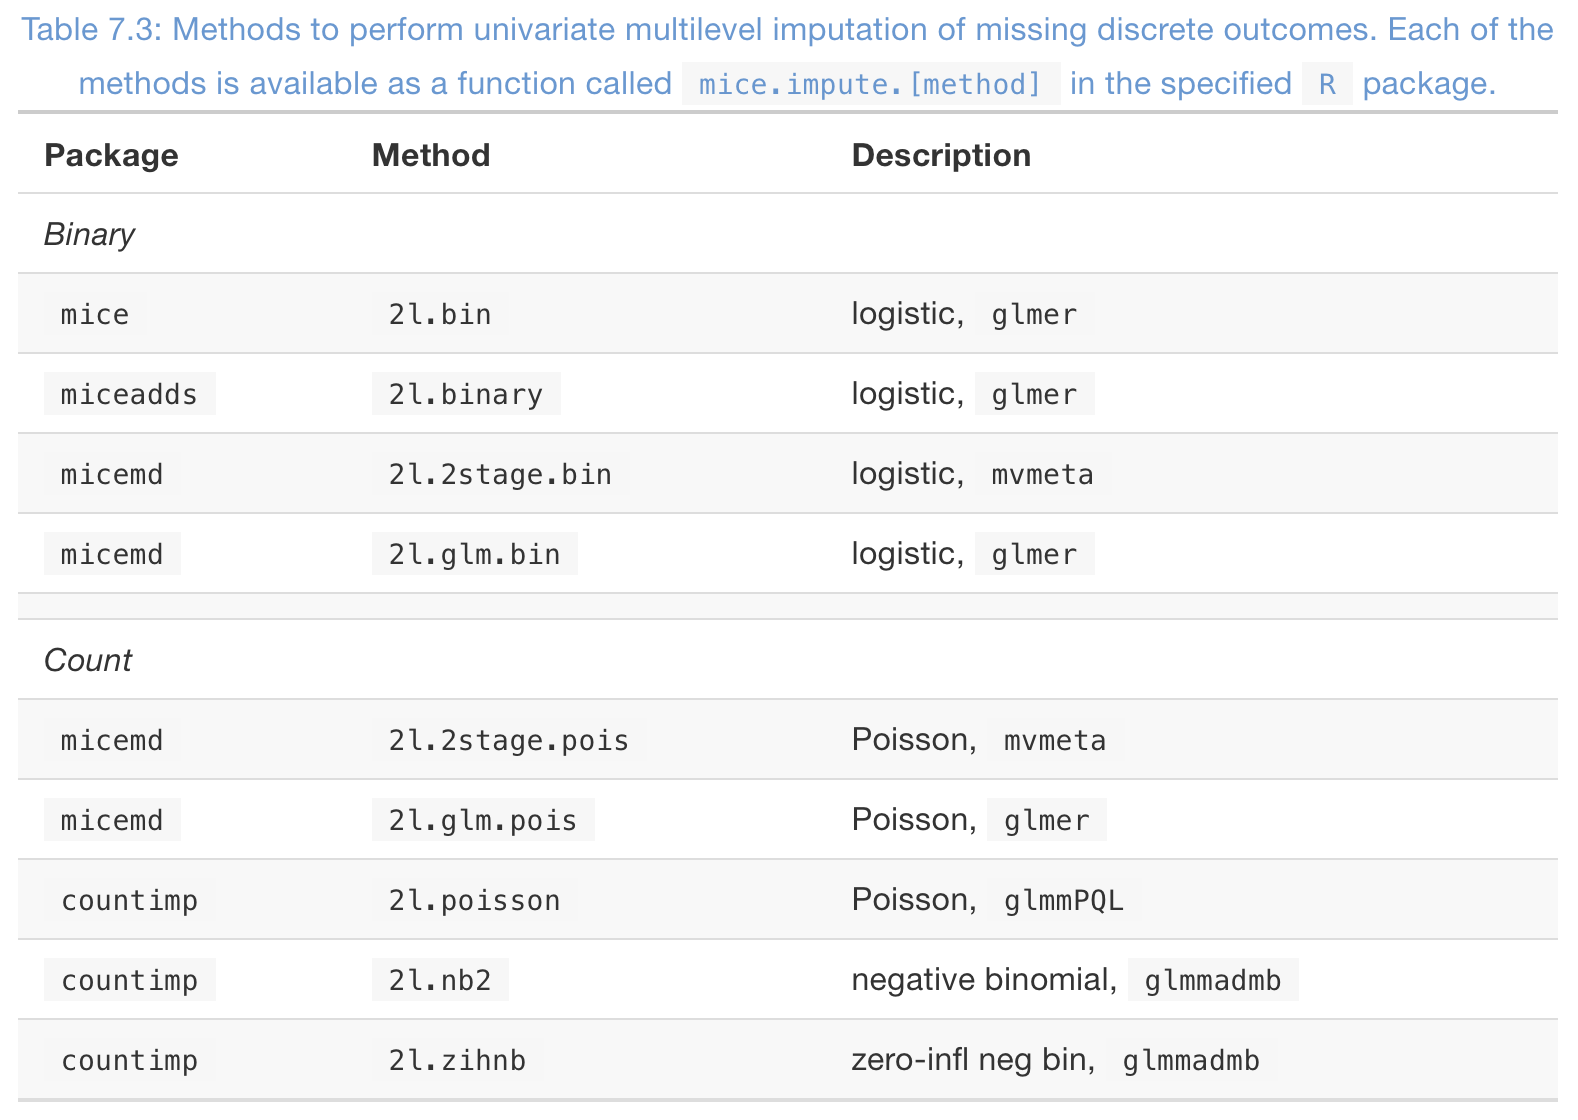
\includegraphics{figures/fig3.png}

\end{frame}

\begin{frame}{Methods for multilevel imputation in \texttt{mice}}
\protect\hypertarget{methods-for-multilevel-imputation-in-mice-2}{}

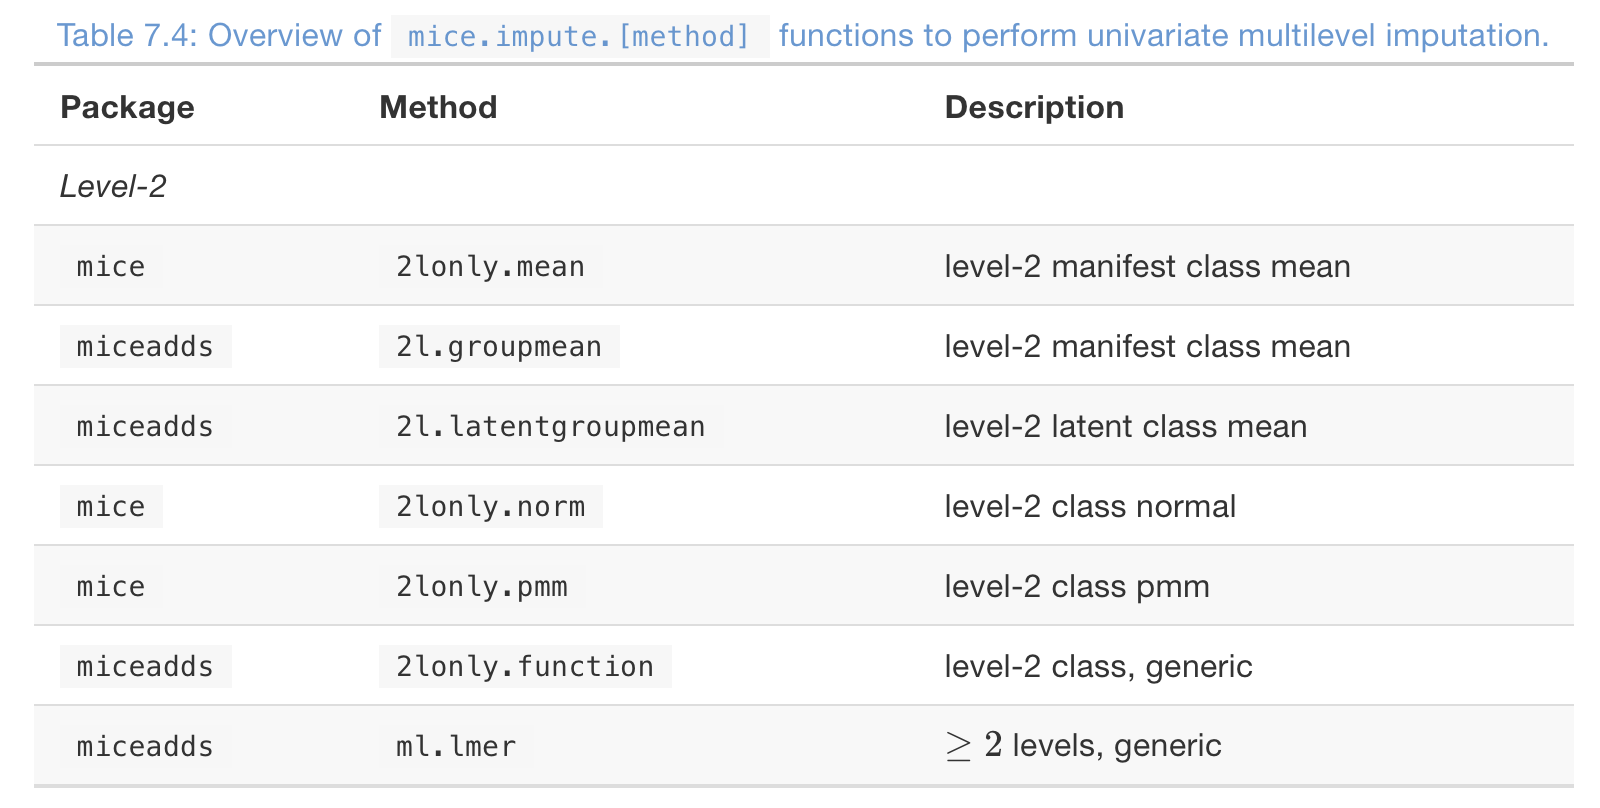
\includegraphics{figures/fig2.png}

\end{frame}

\begin{frame}[fragile]{In practice: start simple, empty model}
\protect\hypertarget{in-practice-start-simple-empty-model}{}

\begin{Shaded}
\begin{Highlighting}[]
\NormalTok{d <-}\StringTok{ }\NormalTok{brandsma[, }\KeywordTok{c}\NormalTok{(}\StringTok{"sch"}\NormalTok{, }\StringTok{"lpo"}\NormalTok{)]}
\NormalTok{pred <-}\StringTok{ }\KeywordTok{make.predictorMatrix}\NormalTok{(d)}
\NormalTok{pred[}\StringTok{"lpo"}\NormalTok{, }\StringTok{"sch"}\NormalTok{] <-}\StringTok{ }\DecValTok{-2}
\NormalTok{imp <-}\StringTok{ }\KeywordTok{mice}\NormalTok{(d, }\DataTypeTok{pred =}\NormalTok{ pred, }\DataTypeTok{meth =} \StringTok{"2l.pmm"}\NormalTok{, }\DataTypeTok{m =} \DecValTok{10}\NormalTok{, }
            \DataTypeTok{maxit =} \DecValTok{1}\NormalTok{, }\DataTypeTok{print =} \OtherTok{FALSE}\NormalTok{, }\DataTypeTok{seed =} \DecValTok{152}\NormalTok{)}
\end{Highlighting}
\end{Shaded}

\end{frame}

\begin{frame}[fragile]{Analysis}
\protect\hypertarget{analysis}{}

\begin{Shaded}
\begin{Highlighting}[]
\KeywordTok{library}\NormalTok{(lme4)}
\end{Highlighting}
\end{Shaded}

\begin{verbatim}
## Loading required package: Matrix
\end{verbatim}

\begin{Shaded}
\begin{Highlighting}[]
\NormalTok{fit <-}\StringTok{ }\KeywordTok{with}\NormalTok{(imp, }\KeywordTok{lmer}\NormalTok{(lpo }\OperatorTok{~}\StringTok{ }\NormalTok{(}\DecValTok{1} \OperatorTok{|}\StringTok{ }\NormalTok{sch), }\DataTypeTok{REML =} \OtherTok{FALSE}\NormalTok{))}
\KeywordTok{summary}\NormalTok{(}\KeywordTok{pool}\NormalTok{(fit))}
\end{Highlighting}
\end{Shaded}

\begin{verbatim}
##             estimate std.error statistic   df p.value
## (Intercept)     40.9     0.322       127 3368       0
\end{verbatim}

\end{frame}

\begin{frame}[fragile]{Variance components}
\protect\hypertarget{variance-components}{}

\begin{Shaded}
\begin{Highlighting}[]
\KeywordTok{library}\NormalTok{(mitml)}
\end{Highlighting}
\end{Shaded}

\begin{verbatim}
## *** This is beta software. Please report any bugs!
## *** See the NEWS file for recent changes.
\end{verbatim}

\begin{Shaded}
\begin{Highlighting}[]
\KeywordTok{testEstimates}\NormalTok{(}\KeywordTok{as.mitml.result}\NormalTok{(fit), }\DataTypeTok{var.comp =} \OtherTok{TRUE}\NormalTok{)}\OperatorTok{$}\NormalTok{var.comp}
\end{Highlighting}
\end{Shaded}

\begin{verbatim}
##                          Estimate
## Intercept~~Intercept|sch   18.021
## Residual~~Residual         63.306
## ICC|sch                     0.222
\end{verbatim}

\end{frame}

\begin{frame}{Now start adding model terms}
\protect\hypertarget{now-start-adding-model-terms}{}

\url{https://stefvanbuuren.name/fimd/sec-mlguidelines.html}

\end{frame}

\begin{frame}[fragile]{Recipe: Missing level-1}
\protect\hypertarget{recipe-missing-level-1}{}

\begin{longtable}[]{@{}ll@{}}
\toprule
& Recipe for a level-1 target\tabularnewline
\midrule
\endhead
1. & Define the most general analytic model to be applied to imputed
data\tabularnewline
2. & Select a \texttt{2l} method that imputes close to the
data\tabularnewline
3. & Include all level-1 variables\tabularnewline
4. & Include the disaggregated cluster means of all level-1
variables\tabularnewline
5. & Include all level-1 interactions implied by the analytic
model\tabularnewline
6. & Include all level-2 predictors\tabularnewline
7. & Include all level-2 interactions implied by the analytic
model\tabularnewline
8. & Include all cross-level interactions implied by the analytic
model\tabularnewline
9. & Include predictors related to the missingness and the
target\tabularnewline
10. & Exclude any terms involving the target\tabularnewline
\bottomrule
\end{longtable}

\end{frame}

\begin{frame}[fragile]{Uncollected variables: conclusion}
\protect\hypertarget{uncollected-variables-conclusion}{}

\begin{itemize}
\tightlist
\item
  No need restrict analysis to least common denominator
\item
  Impute systematically missing data with multilevel imputation model

  \begin{itemize}
  \tightlist
  \item
    Either 2-stage or generalized multilevel
  \end{itemize}
\item
  Technically still challenging, but doable (in \texttt{Stata} or
  \texttt{R})
\item
  More detail: \url{https://stefvanbuuren.name/fimd/ch-multilevel.html}
\end{itemize}

\end{frame}

\begin{frame}{Wrap up}
\protect\hypertarget{wrap-up}{}

\begin{enumerate}
\tightlist
\item
  Different number of categories
\item
  Uncollected variables
\end{enumerate}

\begin{itemize}
\tightlist
\item
  I believe multiple imputation provides substantial progress over

  \begin{itemize}
  \tightlist
  \item
    ad-hoc recoding strategies
  \item
    restriction to observed data
  \end{itemize}
\item
  Of course, we always need MAR assumptions, but these are often natural
  for combined data
\item
  Still experimental, more experience is needed
\item
  Long-term vision: data-combination as a \textbf{information
  translation service} for distributed data
\end{itemize}

\end{frame}

\end{document}
